\documentclass{myreport}

\usepackage{longtable}

% % Change figure (table, section) numbering (e.g., from 'Figure 1' to 'Figure S1')
%  \renewcommand{\thefigure}{S\arabic{figure}}
%  \renewcommand{\thetable}{S\arabic{table}}
%  \renewcommand{\thesection}{S\arabic{section}}
%  \renewcommand{\theequation}{S\arabic{equation}}

\newcommand{\coo}{CO$_2$}
\newcommand{\vcmax}{$V_{\text{cmax}}$}
\newcommand{\jmax}{$J_{\text{max}}$}
\newcommand{\rsq}{$R^2$}

\begin{document}
\pagestyle{headings}

% Document must include
% ---------------------
% 

%% Title
\title{P-model evaluation}

\maketitle

\tableofcontents

%%%%%%%%%%%%%%%%%%%%%%%%%%%%%%%%%%%%%%%%%%%%%%%%%%%%%%%%
\section{Introduction}

Realistic, reliable and robust estimates of photosynthesis are crucial to understand variations in the carbon cycle, monitor forest and cropland productivity, and predict impacts of global environmental change on ecosystem functioning. Understanding how photosynthetic rates depend on temperature, humidity, solar radiation, CO$_2$ and soil moisture is at the core of this challenge and quantitative predictions of photosynthetic CO$_2$ assimilation over a wide range of conditions and spatial scales are the target of a range of photosynthesis models. Most widely used mechanistic photosynthesis models are funded in the Farquhar-von Caemmerer-Berry (FvCB) Model for C3 plants \citep{farquhar80, voncaemmerer81}. This formulation is used as an integral part of practically all Dynamic Vegetation Models (DVMs) and Earth System Models (ESMs) in use today (xxx cite some review?) and, in combination with stomatal conductance ($g_s$) models \citep{ball87, leuning95pce, medlyn11gcb}, couples water and carbon fluxes in and out of stomates at the leaf surface. In its essence, the FvCB model describes the saturating relationship between leaf-internal CO$_2$ concentrations ($c_i$) and assimilation ($A$), and how this relationship depends on absorbed photosynthetically active radiation (APAR). It simulates $A$ as the minimum of a light-limited and a Rubisco-limited assimilation rate. 

Although this can be considered a standard model for leaf-scale photosynthesis, DVM and ESM model results for ecosystem-level fluxes and their response to environmental factors remain divergent \citep{rogers17}. This is, i.a., due to assumptions that have to be made regarding photosynthetic parameters for which the FvCB model itself makes no prediction. This concerns in particular the maximum rate of Rubisco carboxylation (\vcmax\ ) and the maximum rate of electron transport (\jmax\ ) for ribulose-1,5-bisphosphate (RuBP) regeneration, which together determine the relationship between $c_i$ and $A$ in the FvCB model. 

Common approaches for determining the values of \vcmax\ and \jmax\ in DVMs are to prescribe fixed values of \vcmax\ and \jmax\  per plant functional type and attempt to simulate their distribution in space (Sitch et al. 2003) (more refs), or to use empirical relationships between leaf N and \vcmax\ and simulate leaf N internally (refs). While the FvCB model describes a non-linear relationship between (instantaneous) assimilation and absorbed light, it has been known for a long time that ecosystem production, integrated over longer time periods (weeks to months), scales linearly with the APAR (Monteith 1972). This observation underlies the light use efficiency (LUE) model which describes ecosystem-level photosynthesis (gross primary productivity, GPP) as the product of APAR and LUE as
\begin{equation}
\label{eq:luemodel}
\text{GPP} = \text{PAR} \cdot \text{fAPAR} \cdot \text{LUE} \;,
\end{equation}
where PAR is the incident photosynthetically active radiation and fAPAR is the fraction of absorbed PAR. The LUE model serves as a simple and robust basis for a number of observation-driven GPP models that use fAPAR and PAR based on remote sensing data and combine this with different approaches for simulating LUE \citep{running04, zhang17scidat, field95rse}, or for forest growth models \citep{landsberg97fem}. Other remote sensing data-based models \citep{jiang16rse} apply the FvCB model in combination with vegetation cover and type data and prescribed \vcmax\ for a set of plant functional types.

The model described here unifies the two approaches (FvCB and LUE models) by assuming that the photosynthetic machinery tends to coordinate \vcmax\ and \jmax\  in order to operate close to the intersection of the light-limited and Rubisco-limited assimilation rates (\textit{Coordination Hypothesis}, \cite{maire12po}). Daily-to-monthly average assimilation rates can thus be described as linear functions of absorbed PAR in the form of a LUE model (Eq. \ref{eq:lue}). Our model further assumes an optimality principle that balances the C cost of maintaining the transpiration and carboxylation (\vcmax\ ) capacities and thus arrives at a prediction for how \vcmax\ and $g_s$ acclimate to the environment and determine the ratio of leaf-internal to ambient CO$_2$ ($c_i:c_a = \chi$), given temperature ($T$), water vapour pressure deficit (VPD $= D$), atmospheric pressure ($p$) and ambient CO$_2$ concentrations.

Taken together, the model presented here (thereafter referred to as the \textit{P-model}), provides a consistent, optimality-based theory for predicting the acclimation of leaf-level photosynthesis to its environment \citep{prentice14ecollett} and for simulating LUE while relying on a minimum of prescribed parameters \citep{wang17natpl}. In combination with prescribed PAR and remotely sensed fAPAR, it can thus be used to estimate GPP across diverse environmental conditions. Therefore, the P-model has the advantage over other widely used data-driven GPP models (e.g., MODIS, FLUXCOM) in that it accounts for effects by changing CO$_2$, and that it uses first principles to mechanistically resolve effects by $T$, $D$ and $p$, and thereby \textit{predicts} key photosynthetic parameters instead of relying on prescribed values. The theoretical approach is described in more detail in Section \ref{sec:theory} and a full derivation of equations is given in Appendix XXX. 

The theory underlying the P-model has been described before by \cite{prentice14ecollett} and has been used to predict variations of $\chi$ \citep{wang17natpl}, \vcmax\ \citep{smith19ecollett}, and leaf nitrogen \citep{dong16bg} across environmental gradients and to simulate how changes in primary productivity have driven the terrestrial C sink over the past decades \citep{keenan17natcomm}. The purpose of the present paper is two-fold. First, it provides a recapitulation of the P-model`s underlying theory, and provides a complete description and reference for its implementation, along with version-controlled and open access model code (Fortran 90, xxx). A companion paper describes an R package to run the P-model, which provides the software for wrapping its implementation in different languages within a common framework and thereby serves to facilitate the model`s application in a wide variety of contexts and research communities. Second, this paper provides a comprehensive evaluation of the P-model as a LUE model for simulating GPP, using data from flux measurements (FLUXNET Tier 1 dataset). The evaluation focuses on different components of variability (spatial, annual, seasonal, daily anomalies), and the GPP response to soil moisture drought.

Here, we evaluate three P-model versions. The version `ORG' is the P-model in its ``original'' form, as used in \cite{wang17natpl} and \cite{keenan17natcomm}. Note however, that their implementation of the basic equations may differ slightly from the implementation presented here. A temperature-dependence of the quantum yield efficiency, held constant for previous publications using the P-model, was introduced in model version `BRC', based on the formulation given by \cite{bernacchi03pce}. Furthermore, Stocker et al. (2019) (xxx addref) identified a general bias of simulated GPP in the P-model (as well as in other remote sensing-based GPP models) that is closely related to the timing and magnitude of soil moisture effects on LUE. Therefore, we tested an additional P-model version (`FULL') that additionally uses an empirical soil moisture stress function. All versions are benchmarked against a null model (`NULL') where LUE is assumed to be constant in time and uniform across space. An additional null model (`NULLpft') is tested where a constant LUE is assumed for each plant functional types - an approach often employed by remote sensing-based GPP models (xxx ref).

Benchmarking of data-driven models is challenging due to errors introduced by uncertain model forcing data \citep{ryu19rse} (climate and fAPAR data differences between sources) and by uncertainties in observational data used for evaluation. We address these two points here with an additional focus on uncertainties in the fAPAR data, which is used as model forcing (Sec. XXX), and assess the robustness of model evaluation subject to uncertainties in the GPP data, derived from different flux decomposition methods (Sec. XXX). 

Accurately simulating sensitivities of processes to environmental conditions is key for reliable model predictions. However, relying just on continuous, not experimentally disturbed measurements, as done here with FLUXNET data, it's challenging to assess modelled GPP for extreme environmental conditions. Therefore, in addition to evaluating model-observation agreement statistics for GPP variability at different scales (Sec. \ref{sec:evalmethod_variability}), we evaluate the bias of simulated GPP during the course of drought events (Sec. \ref{sec:droughtresponse}).

\section{Theory}
\label{sec:theory}

The theory underlying the P-model has been described by \cite{prentice14ecollett} and \cite{wang17natpl} and the derivation of equations is given therein. It is presented here again for completeness of the present model description. Please cite \cite{wang17natpl} when referring to the model theory. 

\subsection{Balancing carbon and water costs}
\label{sec:watercarbon}
The P-model centers around a prediction for the optimal ratio of leaf-internal to ambient \coo\ concentrations $c_i:c_a$ (termed $\chi$) that balances the costs associated with maintaining the transpiration stream ($E/A$) and the cost of maintaining a given carboxylation capacity ($V_{\mathrm{cmax}}/A$). The optimal balance is achieved when the two marginal costs are equal: 
\begin{equation}
\label{eq:optimality_chi}
a \; \frac{\partial (E/A)}{\partial \chi} = -b \; \frac{\partial (V_{\mathrm{cmax}}/A)}{\partial \chi}\;.
\end{equation}
Here, $a$ and $b$ are the respective unit costs. $b$ is assumed to be constant, and $a$ to scale linearly with the temperature-dependent viscosity of water $\eta(T)$. Below, we use $\beta = b / a'$, with $a = \eta^\ast a'$ and $\eta^\ast = \eta(T) / \eta(25^{\circ}\text{C})$. The optimal $\chi$ solves the above equation. We can use Fick's law \citep{fick1855} to express transpiration and assimilation as a function of stomatal conductance $g_s$: 
\begin{equation}
\label{eq:egs}
    E = 1.6 g_s D
\end{equation}
and 
\begin{equation}
\label{eq:ags}
    A = g_s (1-\chi)   
\end{equation}
and use the Rubisco-limitedassimilation rate from the FvCB model:
\begin{equation}
\label{eq:ac}
A = A_C = V_{\mathrm{cmax}} \; \frac{\chi c_a-\Gamma^{\ast}}{\chi c_a + K}\; ,
\end{equation}
$K$ is the Michaelis-Menten coefficient for Rubisco-limited assimilation (see Sec. \ref{sec:kmm}), and $\Gamma^{\ast}$ is the photorespiratory compensation point in absence of dark respiration (see Sec. \ref{sec:gs}). The optimal $\chi$ can thus be derived as
\begin{equation}
\label{eq:chiopt}
\chi = \frac{\Gamma^{\ast}}{c_a} + \left(1- \frac{\Gamma^{\ast}}{c_a}\right)\;\frac{\xi}{\xi + \sqrt{D}}\;,
\end{equation}
with 
\begin{equation}
\label{eq:xi}
\xi = \sqrt{\frac{\beta (K+\Gamma^{\ast})}{1.6 \eta^{\ast}}}\;.
\end{equation}
See Appendix \ref{app:steps_watercarbon} for intermediate steps. Note that the Coordination Hypothesis has not explicitly been assumed here, but because both terms in Eq. \ref{eq:optimality_chi} are divided by $A$, the solution is independent of whether the Rubisco-limited rate $A_C$ or the light-limited rate $A_J$ (see below) is followed.

With this prediction for $\chi$, the equation for the light-limited assimilation rate from the FvCB model can be used to write
\begin{equation}
\label{eq:aj}
        A_J = \varphi_0 \; I_{\mathrm{abs}}\;\underbrace{\frac{\chi c_a - \Gamma^{\ast}}{\chi c_a + 2\Gamma^{\ast}}}_{m} \;.
\end{equation}
This equation has the form of a LUE model (Eq. \ref{eq:luemodel}) in that $A_J$ scales linearly with $I_{\mathrm{abs}}$. Using Eqs. \ref{eq:xi} and \ref{eq:ciopt}, $m$ can be expressed directly as
\begin{equation}
\label{eq:m_lue}
    m = \frac{c_a - \Gamma^{\ast}}{c_a + 2 \Gamma^{\ast} + 3 \Gamma^{\ast} \sqrt{\frac{1.6 \eta^{\ast} D }{\beta\;(K+\Gamma^{\ast})}}} \;.
\end{equation}
The unit cost ratio $\beta$ has been estimated by \cite{wang17natpl} based on leaf $\delta^{13}$C data and a (constant) value of 146 is used here. Eq. \ref{eq:m_lue} provides the basis for predicting \coo\ assimilation rates in the form of a LUE model (Eq. \ref{eq:luemodel}) from an optimality principle that balances water and carbon costs and that can be expressed as a function of $T$ and $p$ (both affecting $\Gamma^{\ast}$, $K$, and $\eta^\ast$), $D$, and $c_a$. This implicitly assumes that \vcmax\ acclimates so that $A_J=A_C$, or, in other words, to just use the available light under average daytime conditions. Evidence for this coordination was presented by \cite{chen93}, \cite{haxeltine96}, and \cite{maire12po}. 

The prediction of optimal $\chi$ implies a set of corollaries (see Appendix \ref{sec:corollary}). An estimate for stomatal conductance ($g_s$) and the intrinsic water use efficiency (iWUE = $A/g_s$) directly follow from the optimal water-carbon balance (Eq. \ref{eq:optimality_chi}). By assuming $A_J=A_C$, we can further derive \vcmax , as well as dark respiration ($R_d$), which is a function of \vcmax . Note, that \cite{smith19ecollett} used a different approach to introduce effects by \jmax\ limitation, which is not described here.

\subsection{Introducing \jmax\ limitation}
\label{sec:jmax}
Eq. \ref{eq:aj} assumes that the light response of $A$ is linear up to the coordination point. In reality, rates are saturating towards high light levels due to effects by the limited electron transport rate $J$, necessary for the regeneration of ribulose-1,5,- bisphosphate (RuBP), which reaches a maximum \jmax . To account for this effect, Eq. \ref{eq:aj} has to be modified. This is implemented here following the formulation by \cite{smith37}, using a non-rectangular hyperbola relationship between $A_J$ and $I_{\mathrm{abs}}$ to allow for the effect of finite $J_{\mathrm{max}}$:
\begin{equation}
\label{eq:ajlim}
    A_J = \varphi_0 \; I_{\mathrm{abs}} \; m \; \underbrace{ \frac{1}{\sqrt{1+ \left( \frac{4\;\varphi_0\;I_{\mathrm{abs}}}{J_{\mathrm{max}}} \right)^{2}}} }_{L}
\end{equation}
Following this equation, $A_J$ is no longer linear with respect to $I_{\mathrm{abs}}$ and thus does not have the form of a LUE model. However, \jmax\ can be assumed to acclimate on longer time scales to $I_{\mathrm{abs}}$, so that the marginal gain in assimilation $A$ per unit change in \jmax\ is equal to the unit cost of maintaining \jmax .
\begin{equation}
\label{eq:jmaxpartial}
    \frac{\partial A}{\partial J_{\mathrm{max}}} = c 
\end{equation}
The unit cost $c$ is assumed to include the maintenance of light-harvesting complexes and various proteins involved in the electron transport chain. The cost of maintaining a given \jmax\ is thus assumed to scale linearly with \jmax\ and that this proportionality is constant ($c$ is constant). By taking the derivative of Eq. \ref{eq:ajlim} with respect to \jmax\ and re-arranging terms (see Appendix XXX \ref{app:steps_jmaxlim} for intermediate steps), the \jmax\ limitation factor $L$ can be expressed as
\begin{equation}
    L = \sqrt{ 1 - \left( \frac{c^\ast}{m} \right)^{2/3} }
\end{equation}
with $c^\ast = 4c$. Hence, $A_J$ is again expressed as a linear function of absorbed light. $c^\ast$ can be estimated from typical values of \jmax $:$\vcmax $=$ 1.88 \citep{kattge07} and $\chi =$ 0.8 \citep{lloyd94} to $c^\ast = 0.41$ \citep{wang17natpl}. The revised LUE model thus becomes
\begin{equation}
\label{eq:ajlim4}
    A = \varphi_0 \; I_{\mathrm{abs}} \; m'
\end{equation}
with
\begin{equation}
    m' = m \; \sqrt{1 - \left( \frac{c}{m} \right)^{2/3} }
\end{equation}

\section{Methods}
\label{sec:methods}

\subsection{The light use efficiency model}
\label{sec:luemodel}
$A$ is commonly expressed in units mol m$^{-2}$ s$^{-1}$. For the further model description and evaluation, we refer to ecosystem-scale quantities and in mass units of assimilated C and model GPP (g C m$^{-2}$ d$^{-1}$) following Eq. \ref{eq:luemodel}
with 
\begin{align}
    \text{fAPAR} \cdot \text{PPFD} &\mathrel{\widehat{=}} I_{\text{abs}} \\
    \label{eq:lue_identification}
    \text{LUE} &\mathrel{\widehat{=}} \varphi_0(T) \; \beta(\theta) \; m' \; M_C
\end{align}
Here, $M_C$ is the molar mass of carbon (12.0107 g mol$^{-1}$) to convert from molar units to mass units, and PPFD is the photosynthetic photon flux density integrated over a day (mol d$^{-1}$). fAPAR is unitless and integrates across the canopy, i.e., from fluxes per unit leaf area to fluxes per unit ground area. Note that the quantum yield parameter $\varphi_0$ is modelled here to be temperature-dependent, and an additional soil moisture stress factor ($\beta (\theta)$) is included for modelling LUE (see below).

\subsubsection{Temperature dependence}
\label{sec:tempstress}
The temperature dependence of quantum yield efficiency ($\varphi_0(T)$, unitless) is modelled following the temperature dependence of the maximum quantum yield of photosystem II in light-adapted tobacco leaves, determined by \cite{bernacchi03pce} as 
\begin{equation}
\varphi_0(T) = a_L \; b_L \; ( 0.352 + 0.022\;T - 0.00034\;T^2 )
\end{equation}
where $a_L$ is the leaf absorptance, and $b_L$ is the fraction of absorbed light that reaches photosystem II. Here, $(a_L \cdot b_L)$ is treated as a single calibratable parameter (see Section \ref{sec:calib}) and is further referred to as $\widehat{c_L}\equiv a_L\; b_L$. (All calibratable parameters are thereafter indicated by a hat over the symbol.) Note that the temperature dependence of quantum yield efficiency was not accounted for in earlier publications with the P-model \citep{keenan17natcomm, wang17natpl} and $\varphi_0$ was treated as a constant. To test the effect of this temperature dependence on simulated GPP, we conducted alternative simulations, where a constant $\widehat{\varphi_0}$ was calibrated instead (see Sec. \ref{sec:protocol}). Note, that $\varphi_0$  includes the factor $a_L$ for incomplete leaf absorbtance, which is commonly quantified in separation of the quantum yield efficiency and is assumed a value of 0.72-0.88 in models \citep{rogers17}. Calibrated values $\widehat{\varphi_0}$ are accordingly lower than values for the intrinsic quantum yield reported from experimental studies \citep{long93, singsaas01} and should be regarded as an \textit{effective} quantum yield efficiency. Note that an additional temperature dependence is in $m'$ in Eq. \ref{eq:lue_identification}.

\subsubsection{Soil moisture stress}
\label{sec:soilmstress}
$\beta(\theta)$ is a soil moisture stress function. We use results by \cite{stocker18newphyt} to fit a soil moisture stress functions ($\beta(\theta)\simeq\text{fLUE}$) based on two general patterns. First, the functional form of $\beta(\theta)$ can be approximated by a quadratic function that approaches 1 for soil moisture above a certain threshold $\theta^{\ast}$ and held constant at 1 for soil moisture values above that. Here $\theta$ is the plant-available soil water, expressed as a fraction of field capacity. The general form is:
\begin{equation}
\label{eq:soilmstress}
    \beta =
\begin{cases}
    q(\theta - \theta^{\ast})^2 + 1,& \theta \leq \theta^{\ast}\\
    1,              & \theta > \theta^{\ast}
\end{cases}
\end{equation}
Second, the sensitivity of $\beta(\theta)$ to extreme soil dryness ($\theta \rightarrow 0$) is related to the mean aridity. The dryness-related decline in $\beta(\theta)$ is particularly strong in driest climates, whereas a smaller reduction in $\beta(\theta)$ when soil water gets depleted is recorded at intermediate aridity. In the equation above, the sensitivity parameter $q$ is defined by the maximum $\beta$ reduction at low soil moisture $\beta_0\equiv\beta(\theta=\theta_0)$, leading to $q=(\beta_0-1)/(\theta^{\ast}-\theta_0)^2$. Note that $q$ has a negative value. $\beta_0$ is modelled as a linear function of the mean aridity, quantified by the mean annual ratio of actual over potential evapotranspiration (AET/PET):
\begin{equation}
\label{eq:soilmsensitivity}
\beta_0 = \widehat{a_{\theta}} + \widehat{b_{\theta}} (\text{AET}/\text{PET})
\end{equation}
$\widehat{a_{\theta}}$ and $\widehat{b_{\theta}}$ are treated as calibratable parameters. 

Soil moisture ($\theta$), AET, and PET are simulated using the SPLASH model \cite{davis17}, which treats soil water storage as a single bucket and calculates potential evapotranspiration based on Priestly-Taylor. Here, we account for a variable water holding capacity calculated based soil porosity and depth data from SoilGrids (xxx ref, see Appendix XXX).

\subsection{Simulation protocol}
\label{sec:protocol}
To investigate model performance in dependence of alternative choices for model forcing data (defining fAPAR), alternative model setups (variable/fixed soil moisture and temperature effects), and alternative observational target data for calibration (GPP based on different flux decompositions), we conducted multiple simulation sets. Parameters ($\widehat{c_L}$, $\widehat{a_{\theta}}$, and $\widehat{b_{\theta}}$) are calibrated and evaluated against respective observational data for each simulation set separately.

The simulation set ORG corresponds to the model as used in \cite{wang17natpl}. That is, the quantum efficiency of photosynthesis is fixed ($\widehat{\varphi_0}$ is calibrated, instead of $\widehat{c_L}$), and without accounting for soil moisture stress ($\beta (\theta)=1$). The model is forced with fAPAR data based on MODIS FPAR (MCD15A3H), splines of 4-daily values to daily values (see Section \ref{sec:greennessdata}, and is calibrated against GPP data from FLUXNET 2015 based on the nighttime decomposition method ('NT') (see Section \ref{sec:datafiltering}). All simulation setups are described in Tab. \ref{tab:setups}. The simulation set BRC is identical to ORG, except that  $\widehat{\varphi_0}$ is allowed to vary with temperature and $\widehat{c_L}$ is calibrated. In the simulation set FULL, soil moisture stress is additionally accounted for, and $\widehat{c_L}$, $\widehat{a_{\theta}}$, and $\widehat{b_{\theta}}$ are simultaneously calibrated.

All additional simulations account for both temperature and soil moisture effects. The simulation set FULL\textunderscore FPARitp also uses MODIS FPAR data for fAPAR, but applies a linear interpolation to get daily values instead of splines. This is used to investigate whether the smoothed values of the splined data are responsible for the general underestimation of maximum GPP values during the height of the growing season. The simulation set FULL\textunderscore EVI uses MODIS EVI (MOD13Q1), splined to daily from 8-daily data, to assess to which degree model performance depends on fAPAR forcing data. See Section \ref{sec:greennessdata} for more information.

All of the above-mentioned simulates are calibrated against GPP data based on the nighttime flux decomposition method \citep{Reichstein2005-mp}. Additional simulation sets FULL\textunderscore DT, FULL\textunderscore NTsub, and FULL\textunderscore Ty are used to investigate the dependence of (apparent) model performance on the observational data source to which it is calibrated. We use GPP data based on the nighttime decomposition method \citep{Reichstein2005-mp} for FULL\textunderscore NTsub, the daytime decomposition method \citep{lasslop10} for FULL\textunderscore DT, and an alternative decomposition method used for model-data comparison in \cite{wang17natpl} for FULL\textunderscore Ty. The latter method determines a \textit{constant} background respiration rate as the (fitted) asymptote of CO$_2$ exchange fluxes when PPFD tends to zero. Calibration and evaluation of FULL\textunderscore DT, FULL\textunderscore NTsub, and FULL\textunderscore Ty are done only for sites and dates where observational data is given from all three datasets (DT, NT, and Ty), hence the distiction between FULL\textunderscore NTsub and FULL. 


\begin{table}
\resizebox{\textwidth}{!}{%
\begin{tabular}{lllllllll}
	\toprule
    Setup name                 &  fAPAR data              &  GPP      &  Calibration set  &  SM limit.  &  \widehat{\varphi_0} &  \widehat{c_L}    &  $\widehat{a_{\theta}}$  &  $\widehat{b_{\theta}}$   \\
	\midrule
    ORG                        &  FPAR MCD15A3H, spl.     &  NT       &  valid NT data    &  no         &  0.0492 &  --     &  -- & --   \\
    BRC                        &  FPAR MCD15A3H, spl.     &  NT       &  valid NT data    &  no         &  --     &  0.0817 &  -- & --   \\
    FULL                       &  FPAR MCD15A3H, spl.     &  NT       &  valid NT data    &  yes        &  --     &  0.0870 &  0  & 0.685 \\
	\midrule
    FULL\textunderscore FPARitp &  FPAR MCD15A3H, itpl.   &  NT       &  valid NT data    &  yes        &  --     &  0.0846 &  0  & 0.700 \\
    FULL\textunderscore EVI     &  EVI MOD13Q1, spl.      &  NT       &  valid NT data    &  yes        &  --     &  0.1293 &  0  & 0.766 \\
	\midrule
    FULL\textunderscore DT      &  FPAR MCD15A3H, spl.    &  DT       &  valid NT, DT, Ty &  yes        &  --     &  0.0891 & 0   & 0.690 \\
    FULL\textunderscore Ty      &  FPAR MCD15A3H, spl.    &  Ty       &  valid NT, DT, Ty &  yes        &  --     &  0.0868 & 0   & 0.721 \\
    FULL\textunderscore NTsub   &  FPAR MCD15A3H, spl.    &  NT       &  valid NT, DT, Ty &  yes        &  --     &  0.0899 & 0   & 0.690 \\
	\bottomrule
\end{tabular}}
\caption{Model setups. The standard greenness data, used to define the model forcing for fAPAR is MODIS FPAR MCD15A3H, where the original data, given at 4-day intervals, is splined to daily values (see Section \ref{sec:greennessdata}). Alternative greenness forcing data is based on MODIS EVI MOD13Q1, splined (`spl.') from 8-day intervals to daily, and MODIS FPAR MCD15A3H, linearly interpolated (`itpl.') from 4-day intervals to daily. Standard observational GPP data, used for model calibration and evaluation is from FLUXNET 2015 data, based on the nighttime flux decomposition method (`NT' in the table, variable \texttt{GPP\textunderscore NT\textunderscore VUT\textunderscore REF} in FLUXNET 2015 data). Alternative GPP data used based on the daytime flux decomposition method (`DT' in the table, variable \texttt{GPP\textunderscore DT\textunderscore VUT\textunderscore REF}), and based on an alternative method \citep{wang17natpl} (`Ty' in the table). For setups ORG, BRC, FULL, FULL\textunderscore FPARitp, and FULL\textunderscore EVI, data used for the model calibration is from all dates where (cleaned, see Section \ref{sec:datafiltering}) `NT' data is available. For setups FULL\textunderscore DT, FULL\textunderscore Ty, and FULL\textunderscore NTsub, data used for calibration is from all dates where data is available for all methods `DT', `NT', and `Ty'. `SM limit.' refers to whether or not soil moisture limitation (see Section \ref{sec:soilmstress} is accounted for. `QYE(T)' refers to whether the temperature dependence of quantum yield efficiency after \cite{bernacchi03pce} is accounted for. Column `QUE' specifies the calibrated value for quantum yield efficiency ($\varphi$), columns `a' and `b' specify the calibrated values for variables $a_\theta$ and $b_\theta$ in Eq. \ref{eq:soilmsensitivity}.}
\label{tab:setups}
\end{table}

\clearpage

\subsection{Model calibration}
\label{sec:calib}
The model calibration is restricted to the parameters determining the quantum efficiency of photosynthesis ($\widehat{\varphi_0}$ or $\widehat{c_L}$, respectively) and the dependence of the sensitivity of the soil moisture stress function on average aridity, quantified by AET/PET (parameters $\widehat{a_{\theta}}$ and $\widehat{a_{\theta}}$). We used  Generalised Simulated Annealing from the \textit{GenSA} R package \citep{gensa} to search model parameters that minimise the root mean square error (RMSE) between observed and simulated daily GPP values. This algorithm is particularly suited to find global minima of non-linear objective functions and a large number of local minima.

%The model calibration is implemented within the rsofun R package (function \texttt{calib\textunderscore sofun()}, see accompanying paper Stocker et al., XXX).

\subsection{Forcing data}

\subsubsection{fAPAR}
\label{sec:greennessdata}

Different datasets were used to define fAPAR (Eq. \ref{eq:luemodel}). The standard dataset is MODIS FPAR MCD15A3H, from Collection 6 \citep{modis_fpar_6}, which is given at a resolution of 500 m and 4 days. The data was filtered to remove data points where significant clouds were present, suspicious values equal to 1.00, and outliers (outside three times the inter-quartile range). Filtered values were replaced by the mean value for the respective day-of-year. Daily values were derived using a cubic smoothing spline (function \texttt{smooth.spline()} with parameter \texttt{spar=0.01} in R \citep{Rcoreteam}). MODIS EVI MOD13Q1 data, collection 6 \citep{modis_evi_6}, given at a resolution of 250 m and 8 days, was filtered based on the summary quality control flag, removing ``cloudy'' pixels. Gaps were filled and data splined to daily values as for FPAR MOD13Q1. All fAPAR data were downloaded from Google Earth Engine using the \textit{google\textunderscore earth\textunderscore engine\textunderscore subsets} library \citep{gee_subset}. 

\subsubsection{Meteorological data}
\label{sec:ppfd}
All meteorological forcing data is taken from the FLUXNET Tier 1 dataset, which provides data from measurements taken and processed along with the \coo\ flux measurements. The photosynthetic photon flux density PPFD is calculated from shortwave downwelling radiation as $\text{PPFD} = 2.04 \cdot R_{\text{SW}}$, where $R_{\text{SW}}$ is incoming shortwave radiation from daily FLUXNET 2015 data (variable \texttt{SW\textunderscore IN\textunderscore F}). Vapour pressure deficit (VPD, or $D$ in Sec. \ref{sec:theory}) is taken from daily FLUXNET 2015 data (variable \texttt{VPD\textunderscore F}) and represents means over half-hourly data. We use daily air temperature from the FLUXNET 2015 dataset (variable \texttt{T\textunderscore F}), defined as the mean over half-hourly data. Note that this is a simplification, as we are not using leaf temperature and are not using VPD at the leaf surface, which are more directly relevant for photosynthesis but their estimation imply further assumptions. We use precipitation data (variable \texttt{P\textunderscore F}) is used to force the soil moisture model.

\subsection{Calibration and evaluation data}

\subsubsection{Site selection}
We use data from 68 sites for model calibration and 153 sites for evaluation (Fig. \ref{fig:map_sites}). The number of valid daily GPP data points for the calibration set is 160,061 and 260,284 for the evaluation set. The selection of sites used for calibration is based on the reliability of relationships between \coo\ fluxes, co-located greenness data, and meteorological variables. Specifically, we use data from sites used in \cite{stocker18newphyt} to train machine learning models for explaining relationships between LUE and environmental drivers. This led to excluding data from sites where the total number of data points was too low ($<$500 daily data points per site); where flux data appeared to be unreliable, leading to unreliably trained models; and where noise in the greenness data was particularly high. For the evaluation, we used data from all sites, excluding croplands and data seven additional sites where C4 vegetation is known to be present, based on information provided by the FLUXNET meta information. These sites are: AU-How, DE-Kli, FR-Gri, IT-BCi, US-Ne1, US-Ne2, and US-Ne3.

\begin{figure}[!ht]
    \centering
    \includegraphics[width=0.8\textwidth]{fig/map_sites.pdf}
    \caption{Overview of sites selected for model calibration (green dots) and evaluation (green and black dots). All sites and additional information are listed in Tab. \ref{tab:sites}}
    \label{fig:map_sites}
\end{figure}

\label{sec:sites}

\subsubsection{Data filtering}
\label{sec:datafiltering}
GPP predictions by the RS models are compared to daily GPP estimates from the FLUXNET 2015 Tier 1 data set (downloaded on 13 November, 2016). We used GPP based on the nighttime partitioning method \citep{Reichstein2005-mp} (GPP\textunderscore NT\textunderscore VUT\textunderscore REF) and filtered negative daily GPP values, data for which more than 50\% of the half-hourly data are gap-filled and for which the daytime and nighttime partitioning methods (GPP\textunderscore DT\textunderscore VUT\textunderscore REF and GPP\textunderscore NT\textunderscore VUT\textunderscore REF, respectively) are inconsistent, i.e., the upper and lower 2.5\% quantiles of the difference between GPP values quantified by each method. For additional simulation sets, model calibration and evaluation was done using GPP data based on the daytime partitioning method (GPP\textunderscore DT\textunderscore VUT\textunderscore REF) \citep{lasslop10} with analogous filtering steps, and GPP data based on an alternative method that fits a constant ecosystem respiration rate as the net ecosystem exchange under conditions where PPFD tends to zero (FULL\textunderscore Ty, \cite{wang17natpl}). For all calibration and evaluation, we removed data points before the ``MODIS era'', which started on the 18th of February, 2000.

\subsection{Evaluation methods}

\subsubsection{Components of variability}
\label{sec:evalmethod_variability}
Different components of variability are analyzed separately. We separate spatial (mean annual values by site), annual, seasonal (mean by day-of-year), 5-daily, daily, and the variability in daily anomalies from the mean seasonal cycle. The seasonal variability is determined for different climatic zones (following Koeppen-Geiger classification, see Tab. \ref{tab:kgclimate}). Information about the association of sites with climatic zones is extracted from \cite{falge17}. Evaluations per climatic zone are done here only for zones that had at least five different site's data. For each component of variability, we calculate the adjusted coefficient of determination ($R^2_{\text{adj}}$, thereafter referred to as $R^2}$), and the root mean square error (RMSE). Figures of correlations between simulated and observed values additionally present the mean bias, the slope of the linear regression model, and the number of data points ($N$).

\begin{table}
\caption{Description of Koeppen-Geiger climate zones (based on \cite{falge17}) and number of sites for which data is available per climate zone and hemisphere. Only zones with data from more than three sites are shown.} 
\centering
\begin{tabular}{llll}
  \toprule
  Code & $N$ north & $N$ south & Description \\ 
  \midrule
   Aw   & -- & 5 &  Tropical savannah with dry winter \\ 
   BSk  & 5 & -- & Arid steppe cold \\ 
   Cfa  & 11 & -- & Warm temperate fully humid with hot summer \\ 
   Cfb  & 19 & 5 & Warm temperate fully humid with warm summer \\ 
   Csa  & 12 & -- & Warm temperate with dry and hot summer \\ 
   Csb  & 4 & -- & Warm temperate with dry and warm summer \\ 
   Dfb  & 17 & -- & Cold fully humid warm summer \\ 
   Dfc  & 22 & -- & Cold fully humid cold summer \\ 
   ET   & 4 & -- & Polar tundra \\ 
   \bottomrule
  \end{tabular}
  \label{tab:kgclimate}
\end{table}

% \subsubsection{Functional relationships}
% \label{sec:gam}
% Functional relationships between light use efficiency and its predictors considered in the P-model are based on pooled data from all sites and are derived using Generalized Additive Models (GAMs). The procedure applied here is as follows. First, a GAM is trained on observational data using the \texttt{gam()} function from the \textit{mgcv} R package with method REML \citep{mgcv}. Using all date's data pooled, we trained four models using LUE as targets for training, where LUE is quantified using Eq. \ref{eq:luemodel}, based on observed GPP from the three different flux decomposition methods (see Sec. \ref{sec:datafiltering}) and simulated LUE from the P-model. We use tempearature ($T$), VPD ($D$), and soil moisture ($\theta$) as model predictors. The P-model additionally requires elevation and ambient \coo\ as inputs. However, these variables do not vary at short time scales. The trained models are then applied to an evaluation dataset that is constructed separately as follows. For each predictor $i \in (T, D, \theta)$, three vectors $\mathbf{x}_i, \mathbf{x}_j, \mathbf{x}_k$ are constructed. The first ($\mathbf{x}_i$) is an equally spaced sequence of values of predictor $i$, ranging from its minimum to its maximum in the training dataset. The length of $\mathbf{x}_i$ is $N_i=30$. The second and third vectors $\mathbf{x}_j, \mathbf{x}_k$ are constructed by randomly sampling (with replacement) $N_j=N_k=30$ values of predictors $(j,k)\neq i$, respectively, from the training dataset. Then, a matrix is constructed to contain all combinations $(x_{i,l}, x_{j,m}, x_{k,n})$ of elements of the three vectors with $l \in [1,N_i], m \in [1,N_j], n \in [1,N_k]$. Finally, quantiles are calculated for pooled data across predictors $(j,k)$ and all levels of predictor $i$.

\subsubsection{Drought response}
\label{sec:droughtresponse}
The bias in GPP (modelled minus observed) is calculated for each date belonging to drought events identified by \cite{stocker18newphyt} for 32 (xxx check this number, include in table 5) sites (20 days before and 80 days after drought onset are taken). Drought events ("fLUE droughts") are periods of consecutive days where soil moisture, separated from other drivers using neural networks, reduces LUE below a given threshold. The data specifying the timing and duration of drought events was downloaded from \textit{Zenodo} \citep{flue}. We then re-arranged the data to align all drought events at all sites, normalised data to its median value during the ten days before the onset of droughts (normalisation by subtracting median), and computed quantiles per day, where 'day' is defined with respect to the onset of each drought event.

\section{Evaluation results}
\label{sec:results}

\subsection{Variability across scales}

We first evaluate the model performance with respect to pooled data from all 153 sites, forced with splined MODIS FPAR data for fAPAR in Eq. \ref{eq:luemodel}, and evaluated against GPP data based on the NT flux decomposition. Evaluations with respect to alternative choices for fAPAR data and GPP data are presented in Sections \ref{sec:results_greennessdata} and \ref{sec:results_gppdata}. \rsq\ and RMSE values for all model setups are presented in Tables \ref{tab:rsq} and \ref{tab:rmse}.

The differences in the performance of different model setups are similar across all scales. Additional explanatory power is introduced by accounting for the temperature effects on quantum yield efficiency and by simulated soil moisture stress. The FULL setup of the P-model generally achieves the highest \rsq\ values and the lowest RMSE and outperforms the NULL and NULLpft models.


% Version 1.
% \begin{table}
% \centering
% \begin{tabular}{lllllll}
%   \toprule
%   Setup & xdaily & spatial & annual & seasonal & daily\_var \\ 
%   \midrule
%   ORG & 0.65 & 0.58 & 0.57 & 0.67 & 0.23 \\ 
%   BRC & 0.68 & 0.61 & 0.60 & 0.71 & 0.23 \\ 
%   FULL & 0.69 & 0.63 & 0.66 & 0.70 & 0.25 \\ 
%   NULL & 0.65 & 0.59 & 0.55 & 0.69 & 0.22 \\ 
%   \bottomrule
%   \end{tabular}
% \caption{$R^2$ of different models and for different components of variability. Version 1.} 
% \label{tab:rsq}
% \end{table}


 % Version 2.
 % This table is created by eval_pmodel.Rmd, section 'Metrics table'
\begin{table}
\centering
\begin{tabular}{lllllll}
  \toprule
  Setup & 5-daily & Spatial & Annual & Seasonal & var(daily) & var(annual) \\ 
  \midrule
  ORG & 0.67 & 0.62 & 0.57 & 0.69 & 0.25 & 0.06 \\ 
  BRC & 0.70 & 0.66 & 0.62 & 0.73 & 0.26 & 0.06 \\ 
  FULL & 0.73 & 0.70 & 0.70 & 0.74 & 0.28 & 0.09 \\ 
  NULL & 0.68 & 0.64 & 0.58 & 0.71 & 0.25 & 0.04 \\ 
  NULLpft & 0.69 & 0.66 & 0.61 & 0.73 & 0.25 & 0.03 \\ 
  \midrule
  FULL\_FPARitp & 0.71 & 0.70 & 0.70 & 0.74 & 0.25 & 0.09 \\ 
  FULL\_EVI & 0.69 & 0.56 & 0.47 & 0.72 & 0.29 & 0.14 \\ 
  \midrule
  FULL\_DT & 0.66 & 0.69 & 0.70 & 0.65 & 0.30 & 0.08 \\ 
  FULL\_NTsub & 0.68 & 0.70 & 0.70 & 0.68 & 0.30 & 0.09 \\ 
  FULL\_Ty & 0.70 &  &  & 0.69 & 0.49 &  \\ 
  \bottomrule
  \end{tabular}
\caption{$R^2$ of different model setups and for different components of variability.} 
\label{tab:rsq}
\end{table}


% % Version 1.
% \begin{table}
% \centering
% \begin{tabular}{lllllll}
%   \toprule
%   Setup & xdaily & spatial & annual & seasonal & daily\_var \\ 
%   \midrule
%   ORG & 2.29 & 483 & 461 & 2.00 & 1.69 \\ 
%   BRC & 2.18 & 458 & 440 & 1.88 & 1.69 \\ 
%   FULL & 2.14 & 445 & 407 & 1.91 & 1.70 \\ 
%   NULL & 2.28 & 476 & 478 & 1.94 & 1.66 \\ 
%   \bottomrule
%   \end{tabular}
% \caption{RMSE of different models and for different components of variability} 
% \label{tab:rmse}
% \end{table}


 % Version 2. SOMETHING WENT REALLY WRONG. MUCH HIGHER THAN BEFORE.
 % This table is created by eval_pmodel.Rmd, section 'Metrics table'
\begin{table}
\centering
\begin{tabular}{lllllll}
  \toprule
  Setup & 5-daily & Spatial & Annual & Seasonal & var(daily) & var(annual) \\ 
  \midrule
  ORG & 2.20 & 485.62 & 474.46 & 1.92 & 1.60 & 152.91 \\ 
  BRC & 2.09 & 455.58 & 444.06 & 1.80 & 1.61 & 151.65 \\ 
  FULL & 1.99 & 421.49 & 396.48 & 1.74 & 1.61 & 149.90 \\ 
  NULL & 2.18 & 467.83 & 478.06 & 1.85 & 1.56 & 153.16 \\ 
  NULLpft & 2.11 & 452.12 & 461.23 & 1.79 & 1.58 & 154.35 \\ 
  \midrule
  FULL\_FPARitp & 2.08 & 427.46 & 402.94 & 1.77 & 1.71 & 148.96 \\ 
  FULL\_EVI & 2.18 & 523.04 & 535.66 & 1.85 & 1.56 & 143.11 \\ 
  \midrule
  FULL\_DT & 2.04 & 390.45 & 363.55 & 1.94 & 1.73 & 155.03 \\ 
  FULL\_NTsub & 2.01 & 418.65 & 392.20 & 1.90 & 1.73 & 150.76 \\ 
  FULL\_Ty & 1.84 &  &  & 1.75 & 1.37 &  \\ 
  \bottomrule
  \end{tabular}
\caption{Root mean square error (RMSE) of different model setups and for different components of variability.} 
\label{tab:rmse}
\end{table}


\subsubsection{5-day totals}
The P-model, as used in \cite{wang17natpl} (version referred to as ORG), captures 65\% of the variance in observed GPP with data aggregated to 5-day totals (60’450 data points). Model performance both with respect to explained variance ($R^2$) and the RMSE is improved when additionally accounting for effects of temperature on the quantum yield efficiency (BRC, $R^2 = 68$\%), and when additionally factoring in an empirical soil moisture stress function (FULL, $R^2 = 70$\%, Fig. \ref{fig:modobs_xdaily}). The NULL model with temporally constant and spatially uniform LUE, fitted to the data, performed equally well as ORG, but is outperformed by model versions BRC and FULL. All performance statistics are given in Tables \ref{tab:rsq} and \ref{tab:rmse}. A NULL model where LUE is constant but distinguished between vegetation types (NULLpft) performs as well as BRC. 

\begin{figure}[!ht]
    \includegraphics[width=0.48\textwidth]{fig/modobs_xdaily_FULL.pdf}
    \includegraphics[width=0.48\textwidth]{fig/modobs_xdaily_NULL.pdf}
    \caption{Correlation of observed and modelled GPP values of all sites pooled, mean over 5-day periods, for the model versions FULL (left) and NULL (right).}
    \label{fig:modobs_xdaily}
\end{figure}

\subsubsection{Seasonal variations}

Among the components of variability investigated here, seasonal variations are in general most reliably simulated (\rsq : 0.67-0.70 for P-model setups, and \rsq : 0.69 for the NULL model, Fig. \ref{fig:season} and \ref{fig:season2}). The NULL model captures most of the seasonal variability, especially in climate zones Dfb and Dfc (Fully humid, snow in winter), Cfb, and Cfa (Warm temperate, fully humid). This indicates that in respective climates, most of the  seasonal GPP variations are driven by seasonal changes in insolation (PPFD) and vegetetation greenness (fAPAR). Accounting for temperature effects on the quantum yield efficiency resolves part of the overestimation in the early season. Particularly in climate zone Dfb (fully humid, warm summer, snow in winter), a substantial overestimation of GPP in the early season remains in all setups. While vegetation greenness suggests activity, observed GPP starts to increase only with a substantial delay (up to 2 months at some sites, e.g., US-Los). Within climate zone Dfb, this pattern is clearly visible at almost all sites. Interestingly, an early season high bias is largely absent for sites in climate zone Cfb, where in both observations and the model, GPP starts to increase early on and observations are accurately matched by simulations. Notable exceptions are Cfb sites CZ-wet, DE-Hai, and FR-Fon, where the start of the season is simulated too early, similarly as for sites in Dfb (figures by sites are given in the supplementary material XXX).

In climate zones with a marked dry season (Aw, BSk, Csa, and Csb), GPP is strongly overestimated during the dry season in model setups that do not account for soil moisture stress. The NULL model generally yields the largest bias. High VPD during dry periods reduces LUE in the P-model and leads to lower GPP values and a smaller bias in P-model versions. The empirical soil moisture stress function fully eliminates the dryness-related bias in zones Aw, Csa, and Csb and substantially reduces it for sites in zone BSk. Observations suggest that GPP declines to values around zero during dry periods at sites in zone BSk (mostly savannah vegetation and grasslands, see Table \ref{tab:sites}). A remaining bias in the model setup FULL, which includes the soil moisture stress function, is due to the fact that prescribed fAPAR remains relatively high and that the stress function does not decline to zero.

Model setups that do not account for soil moisture stress tend to underestimate peak season GPP more strongly compared to the model setup FULL. This is a direct consequence of the calibration which balances errors across all data points.

Across-site average peak-season maximum GPP is accurately captured by the model setup FULL in all zones shown in Figs. \ref{fig:season} and \ref{fig:season2}, except for a tendency to underestimate values in zones Aw and Cfb, and overestimate values in zone Csa. Site-level evaluations (see Supplementary Information XXX) suggests no clear pattern of the peak-season underestimation in zone Cfb with vegetation type. The overestimation of peak-season GPP in zone Csa is caused by a high bias at sites with evergreen broadleaved vegetation (FR-Pue, IT-Cp2, IT-Cpz), whereas sites with other vegetation types show no consistent peak season bias. 

 \begin{figure}[!ht]
\includegraphics[width=0.45\textwidth]{fig/meandoy_byzone_Aw_south_.pdf}
\includegraphics[width=0.45\textwidth]{fig/meandoy_byzone_BSk_north_.pdf}\\
\includegraphics[width=0.45\textwidth]{fig/meandoy_byzone_Csa_north_.pdf}
\includegraphics[width=0.45\textwidth]{fig/meandoy_byzone_Csb_north_.pdf}\\
\includegraphics[width=0.45\textwidth]{fig/meandoy_byzone_Cfa_north_.pdf}
\includegraphics[width=0.45\textwidth]{fig/meandoy_byzone_Cfb_north_.pdf}\\
    \caption{Seasonal cycle. Observations are given by the black line and grey band, representing the median and 33/66 \% quantiles of all data (multiple sites and years) pooled by climate zone. Coloured lines represent different model setups. The red band represents 33/66 \% quantiles for the model setup `FULL'. The annotation above each plot specifies the climate zone (see Tab. \ref{tab:kgclimate}), and $N$ given in the top right corner gives the number of sites within the respective climate zone for which data was used. Only climate zones are shown here for which data from at least five sites was available.}
    \label{fig:season}
\end{figure}

 \begin{figure}[!ht]
\includegraphics[width=0.45\textwidth]{fig/meandoy_byzone_Cfb_south_.pdf}
\includegraphics[width=0.45\textwidth]{fig/meandoy_byzone_Dfb_north_.pdf}\\
\includegraphics[width=0.45\textwidth]{fig/meandoy_byzone_Dfc_north_.pdf}
%\includegraphics[width=0.45\textwidth]{fig/meandoy_byzone_ET_north_.pdf}
    \caption{Continued from Fig. \ref{fig:season}}
    \label{fig:season2}
\end{figure}

\clearpage

\subsubsection{Spatial and annual variations}

The \rsq\ for annual GPP simulated by the P-model setups ranges from 0.57 (ORG) to 0.7 (FULL). The NULL model achieves an \rsq\ of 0.58. Most of the explanatory power of the different models for predicting annual total GPP stems from their power in predicting between-site (``spatial'') variations (Fig. \ref{fig:modobs_spatialannual}). The \rsq\ for spatial variations ranges from 0.62 (ORG) to 0.7 (FULL), and 0.64 for the NULL model. In contrast, inter-annual  variations (across years within a given site) are poorly simulated (\rsq : 0.06-0.09 for P-model setups, and 0.04 for the NULL model). Interannual variations are generally much smaller than across site variations, which likely adds to the challenge of accurately capturing interannual variations. Interannual GPP variations are generally better captured at sites where the variability is high and in particular at dry sites (site-level plots in SI XXX). 

\begin{figure}[!ht]
    \includegraphics[width=0.48\textwidth]{fig/modobs_spatial_annual_FULL.pdf}
    \includegraphics[width=0.48\textwidth]{fig/modobs_spatial_annual_NULL.pdf}\\
    \includegraphics[width=0.45\textwidth]{fig/modobs_spatial_annual_EVI.pdf}
    \caption{Correlation of modelled and observed annual GPP in simulation FULL (top) and the NULL model (bottom). The red line and text are based on means across years by site and represents spatial (across-site) variations. Black lines and text are based on annual values, one line for each site. Lines represent linear regressions. $R^2$ and RMSE statistics for annual values (black text) are based on pooled data from all sites. For a perfect fit between modelled and observed annual GPP values, all black lines (representing the linear regression model of annual values for a single site) would lie on the 1:1 line and have a slope of 1. The fact that for some sites, the linear regression has a slope that deviates much from 1, or is even negative, is illustrative of the poor model performance in capturing interannual variability.}
    \label{fig:modobs_spatialannual}
\end{figure}


\subsection{Greenness data}

Model predictions are highly sensitive to the greenness data used as model forcing. We investigated to what degree model performance is subject to using alternative greenness forcing data. As alternatives to the standard dataset that we used for all other simulations (MODIS FPAR, splined to daily values), we used MODIS EVI and a linearly interpolated version of MODIS FPAR, and focused on a limited set of aspects of model performance which have been discussed above.

We find that interannual variations are better simulated when using MODIS EVI as a forcing (\rsq : 0.14), compared to MODIS FPAR, splined (\rsq : 0.09). However, spatial variations are better captured when using MODIS FPAR (Fig. \ref{fig:modobs_spatialannual}, \rsq : 0.70), as opposed to the model setup using MODIS EVI (\rsq : 0.56). 

Furthermore, the early season high bias in simulated GPP in zone Dfb appears both when the model is forced by MODIS FPAR, and when forced with MODIS EVI (Fig. \ref{fig:season_greenness}, left). The overestimation of GPP during the dry period in zone BSk is larger when using MODIS EVI than when using MODIS FPAR (Fig. \ref{fig:season_greenness}, right), while peak-season bias of GPP in zones BSk, Cfb, and Csb are similar in both model versions (not shown). EVI and FPAR show somewhat different behaviour depending on vegetation type. The EVI-forced model setup tends to be biased low in evergreen needle-leaved vegetation, and has generally lower values in all evergreen vegetation types compared to the FPAR-forced setup. For other vegetation types, there is no general difference in model bias between the two setups (not shown).

 \begin{figure}[!ht]
    \centering
\includegraphics[width=0.45\textwidth]{fig/meandoy_byzone_Dfb_north_greenness.pdf}
\includegraphics[width=0.45\textwidth]{fig/meandoy_byzone_BSk_north_greenness.pdf}\\
    \caption{Mean seasonal cycle for model setus with different greenness forcing data. Observations are given by the black line and grey band, representing the median and 33/66 \% quantiles of all data (multiple sites and years) pooled by climate zone. Coloured lines represent model setups, forced with different greenness data. The red band represents 33/66 \% quantiles for the model setup `FULL'. The annotation above each plot specifies the climate zone (see Tab. \ref{tab:kgclimate}), and $N$ given in the top right corner gives the number of sites within the respective climate zone for which data was used. Climate zones shown here are illustrative examples.}
    \label{fig:season_greenness}
\end{figure}

\clearpage

\subsection{GPP target data}

Model-data agreement is generally best when the model is compared to GPP data based on the flux decomposition method 'Ty' \citep{wang17natpl}. For GPP aggregated to 5-day totals, the model achieves an \rsq\ of 0.7 when compared to GPP 'Ty', as opposed to 0.66 and 0.68 compared to the DT and NT methods, respectively (Tab. \ref{tab:rsq}, Fig. \ref{fig:modobs_10d_gppdata}). Variations in daily values are much better captured by the model when evaluating to GPP 'Ty' (\rsq : 0.49), as compared to evaluations against DT or NT (\rsq : 0.30). Spatial and annual correlations are not evaluated for GPP Ty due to missing data. Correlations at the 5-day, seasonal and daily time scales rely on dates for which neither the NT, DT, nor Ty method has missing values and thus contain an equal number of data points. Therefore NT evaluations, repeated here, are not identical to the ones above and are referred to as 'NTsub' in Tables \ref{tab:rsq} and \ref{tab:rmse}. 

The different flux decomposition methods make fundamentally different assumptions regarding the sensitivity of ecosystem respiration to diurnal changes in temperature. This should lead to systematic differences in derived observational GPP values and should affect model-data disagreement. As described above, we found a systematic low bias of simulated GPP in the peak-season in the climatic zone Cfb (warm temperate, fully humid, warm summer). We expected that the magnitude of this bias is contingent on the type of GPP data that is used for evaluation. However, as shown in Fig. \ref{fig:season3}, this bias does not seem to be affected by the choice of GPP evaluation data.

 \begin{figure}[!ht]
\includegraphics[width=0.45\textwidth]{fig/meandoy_byzone_Cfb_north_NT.pdf}
\includegraphics[width=0.45\textwidth]{fig/meandoy_byzone_Cfb_north_DT.pdf}\\
\includegraphics[width=0.45\textwidth]{fig/meandoy_byzone_Cfb_north_Ty.pdf}
    \caption{Mean seasonal cycle of simulated (red) observed GPP (black) based on different flux decomposition methods.}
    \label{fig:season3}
\end{figure}

\begin{figure}[!ht]
\includegraphics[width=0.48\textwidth]{fig/modobs_xdaily_NT.pdf}
\includegraphics[width=0.48\textwidth]{fig/modobs_xdaily_DT.pdf}\\
\includegraphics[width=0.48\textwidth]{fig/modobs_xdaily_Ty.pdf}
    \caption{Correlation of observed and modelled GPP values of all sites pooled, mean over 5-day periods, determined from comparing respectively calibrated models to different observational GPP data (based on different flux decomposition methods, `DT' for the daytime method, `NT' for the nighttime method and `Ty' for the method by Davis et al. (xxx unpublished?))}
    \label{fig:modobs_10d_gppdata}
\end{figure}


% \subsection{Functional relationships}

% The evaluation of functional relationships reveals a fundamental difference between observational GPP data based on different flux decomposition methods and its response to temperatures below 15$^{\circ}$C. While the DT and NT-based GPP suggests a strong decline towards low temperatures, the slope of the temperature-GPP relationship doesn't appear to vary strongly for GPP values based on the Ty method. The model is better in line with GPP from the Ty method than with others. 

% \begin{figure}[!ht]
% \includegraphics[width=0.5\textwidth]{fig/functionalrel_gam_temp.pdf}
% \includegraphics[width=0.5\textwidth]{fig/functionalrel_gam_vpd.pdf}\\
% \includegraphics[width=0.5\textwidth]{fig/functionalrel_gam_soilm.pdf}
%     \caption{Functional relationship of LUE in response to temperature, VPD, and soil moisture. Functional relationships in different observational data (`NT', `DT', `Ty') are determined by GAMs. `P-model, GAM' is determined from the model outputs for the same data points as `NT', `DT', and `Ty'. `P-model' is determined from applying the model directly. A more detailed description of the method is given in Section \ref{sec:gam}}
%     \label{fig:functionalrel}
% \end{figure}


\subsection{Drought response}

The model setup BRC, which does not include the empirical soil moisture stress function (Eq. \ref{eq:soilmstress}), systematically overestimates GPP during droughts. This bias has a clear pattern. It increases sharply at the onset of drought events and continues to increase throughout the course of droughts. The bias is strongly reduced by applying the empricial soil moisture stress function in the FULL model setup. Here, 'droughts' are periods where soil moisture is known to reduce the light use efficiency of vegetation, based on the analysis by \cite{stocker18newphyt}.  

\begin{figure}[!ht]
    \centering
\includegraphics[width=0.8\textwidth]{fig/droughtresponse.pdf}
    \caption{Bias in simulated GPP during the course of drought events. Simulated GPP is from a simulation with (FULL) and without (BRC) accounting for soil moisture stress. The timing of drought events is taken from \cite{stocker18newphyt} and is identified by an apparent soil moisture-related reduction of observed light use efficiency at 36 FLUXNET sites. The bias is calculated as simulated minus observed GPP. Data from multiple drought events and sites are aligned by the date of drought onset and aggregated across all sites and events (lines for medians, shaded ranges from the 33\% and 66\% quantiles).}
    \label{fig:modobs_droughtresponse}
\end{figure}

\clearpage

% \subsubsection{VPD}

% Vapour pressure deficit ($D$) is calculated from vapour pressure (CRU) or specific humidity (WATCH-WFDEI) input data. In general, $D$ is the difference between actual and saturation vapour pressure:
% \begin{equation}
%     D = e_a - e_s
% \end{equation}
% We calculate saturation vapour pressure ($e_s$, in Pa) following Allen et al. (2005) as a function of temperature  as
% \begin{equation}
% e_s = 611 \; \exp \left( {\frac{17.27\;T_C}{T_C+237.3}} \right)
% \end{equation}
% $T_C$ is the temperature expressed in units of degrees Celsius. Note that Allen et al. (2005) use 6.108 instead of 6.11. The Python implementation uses daily maximum and daily minimum temperature, which is equivalent to above formulation with $T=(T_{\text{min}}+T_{\text{max}})/2$. $e_a$ is provided by CRU as an input dataset. WATCH-WFDEI provides specific humidity data ($q$), which can be converted to the mass mixing ratio of water vapor to dry air ($w$) (dimensionless) by
% \begin{equation}
%     w = \frac{q}{1-q}
% \end{equation}
% and finally to actual vapour pressure by
% \begin{equation}
%     e_a = P \frac{w R_v}{R_d + w R_v}
% \end{equation}
% where $P$ is the atmospheric pressure (Pa), $R_v$ is the specific gas constant for water vapour and $R_d$ is the specific gas constant for dry air. The specific gas constants are calculated from the universal gas constant $R$ and the molecular mass $M$ as $R_{\text{specific}}=R/M$. ($R$ is 8.3143 J mol$^{-1}$ K$^{-1}$. The molecular mass of dry air is $M_d=$ 28.963 g mol$^{-1}$ and the molecular mass of water vapor is $M_v=$ 18.02 g mol$^{-1}$.) Atmospheric pressure is assumed to be at standard conditions (101325 Pa) corrected for local elevation (barometric formula adopted from SPLASH, Eq. 20 in Davis et al., 2017).




% \begin{table}
% \centering
% \begin{tabular}{ p{1.2cm} p{2.5cm} p{2.5cm} p{4cm} l }
% \multicolumn{5}{l}{\textbf{ WATCH-WFDEI }} \\
% \hline
% \textbf{symbol} & \textbf{variable name} & \textbf{file name} & \textbf{variable description} & \textbf{units} \\
% \hline
% $T$ & \texttt{Tair} & \texttt{Tair\_WFDEI} & 2 m instantaneous air temperature & K \\
% $P_{\text{rain}}$    & \texttt{Rainf}  & \texttt{Rainf\_WFDEI\_CRU} & Rainfall rate, bias corrected with CRU TS3.101 data (TS3.21 for 2010-2012) and gauge ``catch corrected'' (average over previous 3 hrs) & kg m$^{-2}$ s$^{-1}$ \\  
% $P_{\text{snow}}$    & \texttt{Snowf} & \texttt{Snowf\_WFDEI\_CRU} & Snowfall rate, bias corrected with CRU TS3.101 data (TS3.21 for 2010-2012) and gauge ``catch corrected'' (average over previous 3 hrs)  & kg m$^{-2}$ s$^{-1}$ \\  
% $R_{\text{SW}}$    & \texttt{SWdown} & \texttt{SWdown\_WFDEI} & Short-wave downwards surface radiation flux (average over previous 3 hours) & W m$^{-2}$ \\  
% $q$    & \texttt{Qair} & \texttt{Qair\_WFDEI} & 2 m instantaneous specific humidity & kg kg$^{-1}$ \\  
% $p$    & \texttt{PSurf} & \texttt{PSurf\_WFDEI} & Instantaneous surface pressure & Pa \\ 
% \hline
% \end{tabular}
% \caption{Variables used from WATCH-WFDEI meteorological data.}
% \label{tab:meteovars}
% \end{table}

\section{Discussion}

\subsection{Daily anomalies}

 \begin{figure}[!ht]
    \centering
%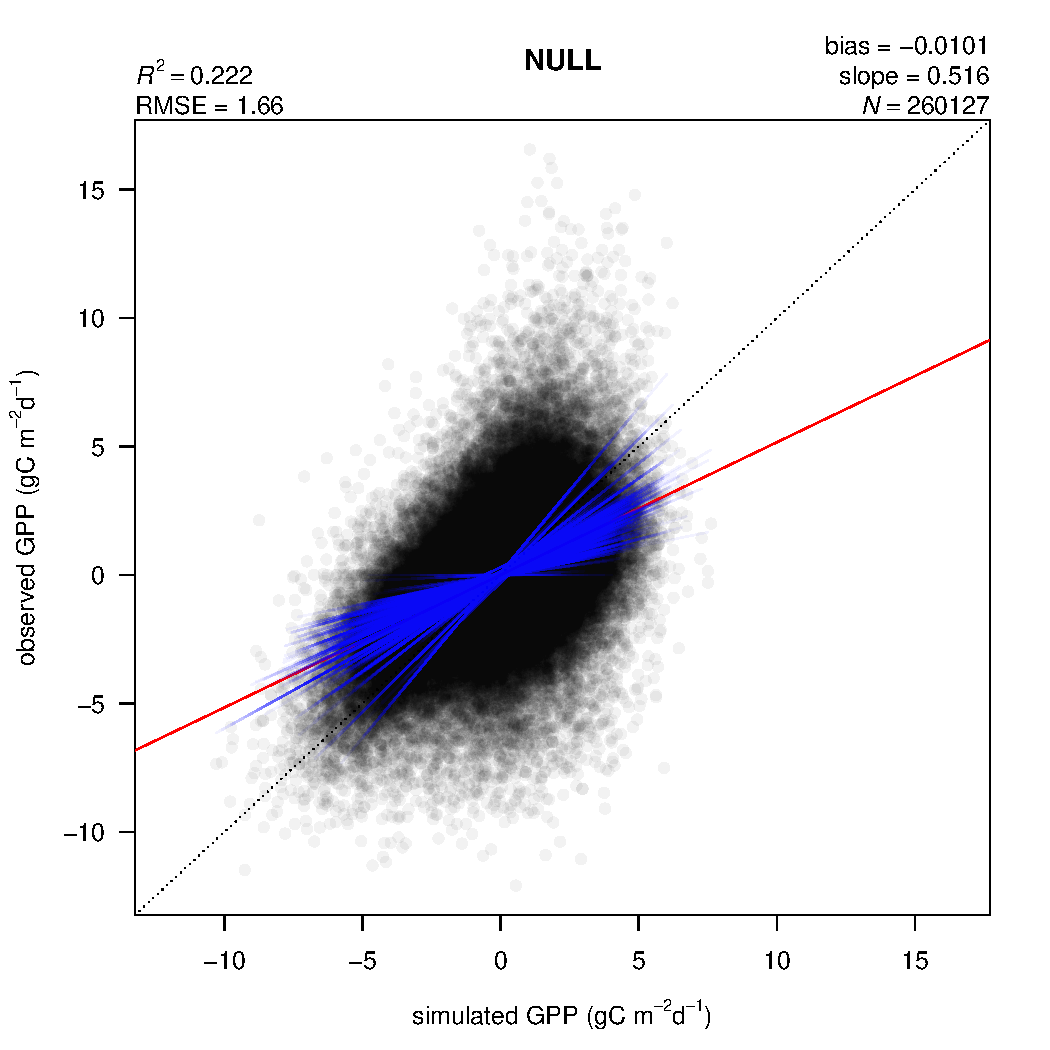
\includegraphics[width=0.4\textwidth]{fig/modobs_anomalies_daily_NULL.pdf}
%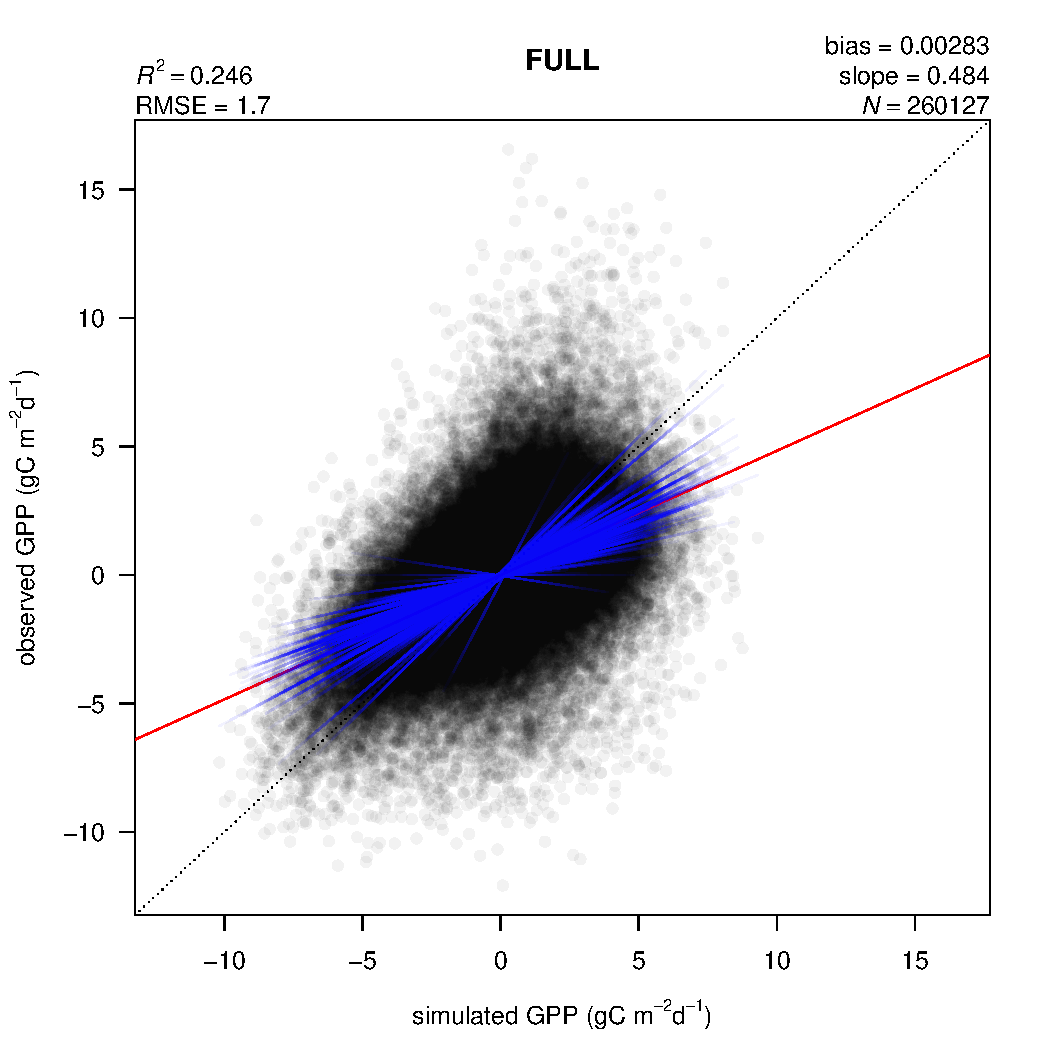
\includegraphics[width=0.4\textwidth]{fig/modobs_anomalies_daily_FULL.pdf}\\
\includegraphics[width=0.4\textwidth]{fig/hist_anomalies_daily_NULL.pdf}
\includegraphics[width=0.4\textwidth]{fig/hist_anomalies_daily_FULL.pdf}
    \caption{Daily anomalies from the mean seasonal cycle. Top row: The cloud of points illustrates daily anomalies from the mean seasonal cycle, blue lines are linear regressions for each site, and the red line is the linear regression of all data pooled. Bottom row: Histogram of daily anomalies from the mean seasonal cycle in the respective model and observations.}
    \label{fig:modobs_anomalies}
\end{figure}


\subsection{Green vegetation cover}



\clearpage


\section{Appendix}

% This table is created by 
\begin{longtable}{lllllllll}
  \toprule
Site & Lon. & Lat. & Period & Veg. & Clim. & N & Calib. & Reference \\ 
  \midrule
  AR-SLu & -66.46 & -33.46 & 2009-2011 & MF & Bwk & 446 &  & \cite{AR-SLu} \\ 
  AR-Vir & -56.19 & -28.24 & 2009-2012 & ENF & Csb & 749 & Y & \cite{AR-Vir} \\ 
  AT-Neu & 11.32 & 47.12 & 2002-2012 & GRA & Dfc & 3243 &  & \cite{AT-Neu} \\ 
  AU-Ade & 131.12 & -13.08 & 2007-2009 & WSA & Aw & 532 & Y & \cite{AU-Ade} \\ 
  AU-ASM & 133.25 & -22.28 & 2010-2013 & ENF & BSh & 1045 & Y & \cite{AU-ASM} \\ 
  AU-Cpr & 140.59 & -34.00 & 2010-2014 & SAV & BSk & 1370 &  & \cite{AU-Cpr} \\ 
  AU-Cum & 150.72 & -33.61 & 2012-2014 & EBF & Cfa & 744 &  & \cite{AU-Cum} \\ 
  AU-DaP & 131.32 & -14.06 & 2007-2013 & GRA & Aw & 1402 & Y & \cite{AU-DaP} \\ 
  AU-DaS & 131.39 & -14.16 & 2008-2014 & SAV & Aw & 2265 & Y & \cite{AU-DaS} \\ 
  AU-Dry & 132.37 & -15.26 & 2008-2014 & SAV & Aw & 1598 & Y & \cite{AU-Dry} \\ 
  AU-Emr & 148.47 & -23.86 & 2011-2013 & GRA & Bwk & 755 &  & \cite{AU-Emr} \\ 
  AU-Fog & 131.31 & -12.55 & 2006-2008 & WET & Aw & 878 & Y & \cite{AU-Fog} \\ 
  AU-Gin & 115.71 & -31.38 & 2011-2014 & WSA & Csa & 942 & Y & \cite{AU-Gin} \\ 
  AU-GWW & 120.65 & -30.19 & 2013-2014 & SAV & Bwk & 663 &  & \cite{AU-GWW} \\ 
  AU-Lox & 140.66 & -34.47 & 2008-2009 & DBF & Bsh & 273 &  & \cite{AU-Lox} \\ 
  AU-RDF & 132.48 & -14.56 & 2011-2013 & WSA & Bwh & 431 &  & \cite{AU-RDF} \\ 
  AU-Rig & 145.58 & -36.65 & 2011-2014 & GRA & Cfb & 1130 &  & \cite{AU-Rig} \\ 
  AU-Rob & 145.63 & -17.12 & 2014-2014 & EBF & Csb & 337 &  & \cite{AU-Rob} \\ 
  AU-Stp & 133.35 & -17.15 & 2008-2014 & GRA & BSh & 1318 & Y & \cite{AU-Stp} \\ 
  AU-TTE & 133.64 & -22.29 & 2012-2013 & OSH & BWh &  94 &  & \cite{AU-TTE} \\ 
  AU-Tum & 148.15 & -35.66 & 2001-2014 & EBF & Cfb & 4335 &  & \cite{AU-Tum} \\ 
  AU-Wac & 145.19 & -37.43 & 2005-2008 & EBF & Cfb & 979 &  & \cite{AU-Wac} \\ 
  AU-Whr & 145.03 & -36.67 & 2011-2014 & EBF & Cfb & 1065 & Y & \cite{AU-Whr} \\ 
  AU-Wom & 144.09 & -37.42 & 2010-2012 & EBF & Cfb & 934 & Y & \cite{AU-Wom} \\ 
  AU-Ync & 146.29 & -34.99 & 2012-2014 & GRA & BSk & 392 &  & \cite{AU-Ync} \\ 
  BE-Bra & 4.52 & 51.31 & 1996-2014 & MF & Cfb & 4208 & Y & \cite{BE-Bra} \\ 
  BE-Vie & 6.00 & 50.31 & 1996-2014 & MF & Cfb & 4733 & Y & \cite{BE-Vie} \\ 
  BR-Sa3 & -54.97 & -3.02 & 2000-2004 & EBF & Am & 1206 &  & \cite{BR-Sa3} \\ 
  CA-Man & -98.48 & 55.88 & 1994-2008 & ENF & Dfc & 1411 &  & \cite{CA-Man} \\ 
  CA-NS1 & -98.48 & 55.88 & 2001-2005 & ENF & Dfc & 771 &  & \cite{CA-NS1} \\ 
  CA-NS2 & -98.52 & 55.91 & 2001-2005 & ENF & Dfc & 873 &  & \cite{CA-NS2} \\ 
  CA-NS3 & -98.38 & 55.91 & 2001-2005 & ENF & Dfc & 1069 &  & \cite{CA-NS3} \\ 
  CA-NS4 & -98.38 & 55.91 & 2002-2005 & ENF & Dfc & 610 &  & \cite{CA-NS4} \\ 
  CA-NS5 & -98.48 & 55.86 & 2001-2005 & ENF & Dfc & 912 &  & \cite{CA-NS5} \\ 
  CA-NS6 & -98.96 & 55.92 & 2001-2005 & OSH & Dfc & 913 &  & \cite{CA-NS6} \\ 
  CA-NS7 & -99.95 & 56.64 & 2002-2005 & OSH & Dfc & 709 &  & \cite{CA-NS7} \\ 
  CA-Qfo & -74.34 & 49.69 & 2003-2010 & ENF & Dfc & 1812 &  & \cite{CA-Qfo} \\ 
  CA-SF1 & -105.82 & 54.48 & 2003-2006 & ENF & Dfc & 525 &  & \cite{CA-SF1} \\ 
  CA-SF2 & -105.88 & 54.25 & 2001-2005 & ENF & Dfc & 675 &  & \cite{CA-SF2} \\ 
  CA-SF3 & -106.01 & 54.09 & 2001-2006 & OSH & Dfc & 651 &  & \cite{CA-SF3} \\ 
  CH-Cha & 8.41 & 47.21 & 2005-2014 & GRA & Cfb & 2885 &  & \cite{CH-Cha} \\ 
  CH-Dav & 9.86 & 46.82 & 1997-2014 & ENF & ET & 4444 &  & \cite{CH-Dav} \\ 
  CH-Fru & 8.54 & 47.12 & 2005-2014 & GRA & Cfb & 2566 & Y & \cite{CH-Fru} \\ 
  CH-Lae & 8.37 & 47.48 & 2004-2014 & MF & Cfb & 3204 & Y & \cite{CH-Lae} \\ 
  CH-Oe1 & 7.73 & 47.29 & 2002-2008 & GRA & Cfb & 2104 & Y & \cite{CH-Oe1} \\ 
  CN-Cha & 128.10 & 42.40 & 2003-2005 & MF & Dwb & 982 &  & \cite{CN-Cha} \\ 
  CN-Cng & 123.51 & 44.59 & 2007-2010 & GRA & Bsh & 1113 & Y & \cite{CN-Cng} \\ 
  CN-Dan & 91.07 & 30.50 & 2004-2005 & GRA & ET & 647 &  & \cite{CN-Dan} \\ 
  CN-Din & 112.54 & 23.17 & 2003-2005 & EBF & Cfa & 917 &  & \cite{CN-Din} \\ 
  CN-Du2 & 116.28 & 42.05 & 2006-2008 & GRA & Dwb & 616 &  & \cite{CN-Du2} \\ 
  CN-Ha2 & 101.33 & 37.61 & 2003-2005 & WET & ET & 1030 &  & \cite{CN-Ha2} \\ 
  CN-HaM & 101.18 & 37.37 & 2002-2004 & GRA &  & 688 &  & \cite{CN-HaM} \\ 
  CN-Qia & 115.06 & 26.74 & 2003-2005 & ENF & Cfa & 992 & Y & \cite{CN-Qia} \\ 
  CN-Sw2 & 111.90 & 41.79 & 2010-2012 & GRA & Bsh & 237 &  & \cite{CN-Sw2} \\ 
  CZ-BK1 & 18.54 & 49.50 & 2004-2008 & ENF & Dfb & 1100 &  & \cite{CZ-BK1} \\ 
  CZ-BK2 & 18.54 & 49.49 & 2004-2006 & GRA & Dfb & 161 &  & \cite{CZ-BK2} \\ 
  CZ-wet & 14.77 & 49.02 & 2006-2014 & WET & Cfb & 2605 & Y & \cite{CZ-wet} \\ 
  DE-Gri & 13.51 & 50.95 & 2004-2014 & GRA & Cfb & 3387 & Y & \cite{DE-Gri} \\ 
  DE-Hai & 10.45 & 51.08 & 2000-2012 & DBF & Cfb & 3435 & Y & \cite{DE-Hai} \\ 
  DE-Lkb & 13.30 & 49.10 & 2009-2013 & ENF & Cfb & 1001 &  & \cite{DE-Lkb} \\ 
  DE-Obe & 13.72 & 50.78 & 2008-2014 & ENF & Cfb & 2043 & Y & \cite{DE-Obe} \\ 
  DE-RuR & 6.30 & 50.62 & 2011-2014 & GRA & Cfb & 1195 & Y & \cite{DE-RuR} \\ 
  DE-SfN & 11.33 & 47.81 & 2012-2014 & WET & Cfb & 750 &  & \cite{DE-SfN} \\ 
  DE-Spw & 14.03 & 51.89 & 2010-2014 & WET & Cfb & 1339 & Y & \cite{DE-Spw} \\ 
  DE-Tha & 13.57 & 50.96 & 1996-2014 & ENF & Cfb & 4887 & Y & \cite{DE-Tha} \\ 
  DK-NuF & -51.39 & 64.13 & 2008-2014 & WET & ET & 882 & Y & \cite{DK-NuF} \\ 
  DK-Sor & 11.64 & 55.49 & 1996-2014 & DBF & Cfb & 4483 & Y & \cite{DK-Sor} \\ 
  DK-ZaF & -20.55 & 74.48 & 2008-2011 & WET & ET & 381 &  & \cite{DK-ZaF} \\ 
  DK-ZaH & -20.55 & 74.47 & 2000-2014 & GRA & ET & 1696 &  & \cite{DK-ZaH} \\ 
  ES-LgS & -2.97 & 37.10 & 2007-2009 & OSH & Csa & 794 &  & \cite{ES-LgS} \\ 
  ES-Ln2 & -3.48 & 36.97 & 2009-2009 & OSH & Csa &  69 &  & \cite{ES-Ln2} \\ 
  FI-Hyy & 24.30 & 61.85 & 1996-2014 & ENF & Dfc & 4222 & Y & \cite{FI-Hyy} \\ 
  FI-Lom & 24.21 & 68.00 & 2007-2009 & WET & Dfc & 575 &  & \cite{FI-Lom} \\ 
  FI-Sod & 26.64 & 67.36 & 2001-2014 & ENF & Dfc & 2816 & Y & \cite{FI-Sod} \\ 
  FR-Fon & 2.78 & 48.48 & 2005-2014 & DBF & Cfb & 2827 & Y & \cite{FR-Fon} \\ 
  FR-LBr & -0.77 & 44.72 & 1996-2008 & ENF & Cfb & 2800 & Y & \cite{FR-LBr} \\ 
  FR-Pue & 3.60 & 43.74 & 2000-2014 & EBF & Csa & 4723 & Y & \cite{FR-Pue} \\ 
  GF-Guy & -52.92 & 5.28 & 2004-2014 & EBF & Af & 3719 &  & \cite{GF-Guy} \\ 
  IT-CA1 & 12.03 & 42.38 & 2011-2014 & DBF & Csa & 1036 &  & \cite{IT-CA1} \\ 
  IT-CA3 & 12.02 & 42.38 & 2011-2014 & DBF & Csa & 913 &  & \cite{IT-CA3} \\ 
  IT-Col & 13.59 & 41.85 & 1996-2014 & DBF & Cfa & 2822 & Y & \cite{IT-Col} \\ 
  IT-Cp2 & 12.36 & 41.70 & 2012-2014 & EBF & Csa & 764 & Y & \cite{IT-Cp2} \\ 
  IT-Cpz & 12.38 & 41.71 & 1997-2009 & EBF & Csa & 2601 & Y & \cite{IT-Cpz} \\ 
  IT-Isp & 8.63 & 45.81 & 2013-2014 & DBF & Cfb & 588 & Y & \cite{IT-Isp} \\ 
  IT-Lav & 11.28 & 45.96 & 2003-2014 & ENF & Cfb & 3919 & Y & \cite{IT-Lav} \\ 
  IT-MBo & 11.05 & 46.01 & 2003-2013 & GRA & Dfb & 3236 & Y & \cite{IT-MBo} \\ 
  IT-Noe & 8.15 & 40.61 & 2004-2014 & CSH & Cwb & 3083 & Y & \cite{IT-Noe} \\ 
  IT-PT1 & 9.06 & 45.20 & 2002-2004 & DBF & Cfa & 828 & Y & \cite{IT-PT1} \\ 
  IT-Ren & 11.43 & 46.59 & 1998-2013 & ENF & Dfc & 3043 & Y & \cite{IT-Ren} \\ 
  IT-Ro2 & 11.92 & 42.39 & 2002-2012 & DBF & Csa & 2671 &  & \cite{IT-Ro2} \\ 
  IT-SR2 & 10.29 & 43.73 & 2013-2014 & ENF & Csa & 668 & Y & \cite{IT-SR2} \\ 
  IT-SRo & 10.28 & 43.73 & 1999-2012 & ENF & Csa & 3791 & Y & \cite{IT-SRo} \\ 
  IT-Tor & 7.58 & 45.84 & 2008-2014 & GRA & Dfc & 1487 & Y & \cite{IT-Tor} \\ 
  JP-MBF & 142.32 & 44.39 & 2003-2005 & DBF & Dfb & 471 &  & \cite{JP-MBF} \\ 
  JP-SMF & 137.08 & 35.26 & 2002-2006 & MF & Cfa & 1288 & Y & \cite{JP-SMF} \\ 
  NL-Hor & 5.07 & 52.24 & 2004-2011 & GRA & Cfb & 2131 & Y & \cite{NL-Hor} \\ 
  NL-Loo & 5.74 & 52.17 & 1996-2013 & ENF & Cfb & 4507 & Y & \cite{NL-Loo} \\ 
  NO-Adv & 15.92 & 78.19 & 2011-2014 & WET & ET & 151 &  & \cite{NO-Adv} \\ 
  NO-Blv & 11.83 & 78.92 & 2008-2009 & SNO & ET & 112 &  & \cite{NO-Blv} \\ 
  RU-Che & 161.34 & 68.61 & 2002-2005 & WET & Dfc & 313 &  & \cite{RU-Che} \\ 
  RU-Cok & 147.49 & 70.83 & 2003-2014 & OSH & Dfc & 985 &  & \cite{RU-Cok} \\ 
  RU-Fyo & 32.92 & 56.46 & 1998-2014 & ENF & Dfb & 4042 & Y & \cite{RU-Fyo} \\ 
  RU-Ha1 & 90.00 & 54.73 & 2002-2004 & GRA & Dfc & 519 &  & \cite{RU-Ha1} \\ 
  SD-Dem & 30.48 & 13.28 & 2005-2009 & SAV & BWh & 762 & Y & \cite{SD-Dem} \\ 
  SN-Dhr & -15.43 & 15.40 & 2010-2013 & SAV & BWh & 686 & Y & \cite{SN-Dhr} \\ 
  US-AR1 & -99.42 & 36.43 & 2009-2012 & GRA & Cfa & 1011 &  & \cite{US-AR1} \\ 
  US-AR2 & -99.60 & 36.64 & 2009-2012 & GRA & Cfa & 882 &  & \cite{US-AR2} \\ 
  US-ARb & -98.04 & 35.55 & 2005-2006 & GRA & Cfa & 414 &  & \cite{US-ARb} \\ 
  US-ARc & -98.04 & 35.55 & 2005-2006 & GRA & Cfa & 488 &  & \cite{US-ARc} \\ 
  US-Blo & -120.63 & 38.90 & 1997-2007 & ENF & Csb & 1827 &  & \cite{US-Blo} \\ 
  US-Cop & -109.39 & 38.09 & 2001-2007 & GRA & BSk & 1067 &  & \cite{US-Cop} \\ 
  US-GBT & -106.24 & 41.37 & 1999-2006 & ENF & Dfc & 541 &  & \cite{US-GBT} \\ 
  US-GLE & -106.24 & 41.37 & 2004-2014 & ENF & Dfb & 2254 & Y & \cite{US-GLE} \\ 
  US-Ha1 & -72.17 & 42.54 & 1991-2012 & DBF & Dfb & 3259 & Y & \cite{US-Ha1} \\ 
  US-KS2 & -80.67 & 28.61 & 2003-2006 & CSH & Cfa & 1263 &  & \cite{US-KS2} \\ 
  US-Los & -89.98 & 46.08 & 2000-2014 & WET & Dfb & 2071 & Y & \cite{US-Los} \\ 
  US-Me1 & -121.50 & 44.58 & 2004-2005 & ENF & Csb & 287 &  & \cite{US-Me1} \\ 
  US-Me2 & -121.56 & 44.45 & 2002-2014 & ENF & Csb & 3525 & Y & \cite{US-Me2} \\ 
  US-Me6 & -121.61 & 44.32 & 2010-2014 & ENF & Csb & 1283 &  & \cite{US-Me6} \\ 
  US-MMS & -86.41 & 39.32 & 1999-2014 & DBF & Cfa & 3524 & Y & \cite{US-MMS} \\ 
  US-Myb & -121.77 & 38.05 & 2010-2014 & WET & Csb & 1153 &  & \cite{US-Myb} \\ 
  US-NR1 & -105.55 & 40.03 & 1998-2014 & ENF & Dfc & 4084 &  & \cite{US-NR1} \\ 
  US-PFa & -90.27 & 45.95 & 1995-2014 & MF & Dfb & 3679 &  & \cite{US-PFa} \\ 
  US-Prr & -147.49 & 65.12 & 2010-2013 & ENF & Dfc & 546 &  & \cite{US-Prr} \\ 
  US-SRG & -110.83 & 31.79 & 2008-2014 & GRA & BSk & 2146 & Y & \cite{US-SRG} \\ 
  US-SRM & -110.87 & 31.82 & 2004-2014 & WSA & BSk & 3093 & Y & \cite{US-SRM} \\ 
  US-Syv & -89.35 & 46.24 & 2001-2014 & MF & Dfb & 2045 & Y & \cite{US-Syv} \\ 
  US-Ton & -120.97 & 38.43 & 2001-2014 & WSA & Csa & 4321 & Y & \cite{US-Ton} \\ 
  US-Tw1 & -121.65 & 38.11 & 2012-2014 & WET & Csa & 688 &  & \cite{US-Tw1} \\ 
  US-Tw4 & -121.64 & 38.10 & 2013-2014 & WET & Csa & 325 &  & \cite{US-Tw4} \\ 
  US-UMB & -84.71 & 45.56 & 2000-2014 & DBF & Dfb & 4015 & Y & \cite{US-UMB} \\ 
  US-UMd & -84.70 & 45.56 & 2007-2014 & DBF & Dfb & 2050 & Y & \cite{US-UMd} \\ 
  US-Var & -120.95 & 38.41 & 2000-2014 & GRA & Csa & 2981 & Y & \cite{US-Var} \\ 
  US-WCr & -90.08 & 45.81 & 1999-2014 & DBF & Dfb & 2333 & Y & \cite{US-WCr} \\ 
  US-Whs & -110.05 & 31.74 & 2007-2014 & OSH & BSk & 1561 &  & \cite{US-Whs} \\ 
  US-Wi0 & -91.08 & 46.62 & 2002-2002 & ENF & Dfb & 228 &  & \cite{US-Wi0} \\ 
  US-Wi3 & -91.10 & 46.63 & 2002-2004 & DBF & Dfb & 415 &  & \cite{US-Wi3} \\ 
  US-Wi4 & -91.17 & 46.74 & 2002-2005 & ENF & Dfb & 712 & Y & \cite{US-Wi4} \\ 
  US-Wi6 & -91.30 & 46.62 & 2002-2003 & OSH & Dfb & 351 &  & \cite{US-Wi6} \\ 
  US-Wi9 & -91.08 & 46.62 & 2004-2005 & ENF & Dfb & 302 &  & \cite{US-Wi9} \\ 
  US-Wkg & -109.94 & 31.74 & 2004-2014 & GRA & BSk & 2676 &  & \cite{US-Wkg} \\ 
  ZA-Kru & 31.50 & -25.02 & 2000-2010 & SAV & BSh & 2124 &  & \cite{ZA-Kru} \\ 
  ZM-Mon & 23.25 & -15.44 & 2000-2009 & DBF & Aw & 641 & Y & \cite{ZM-Mon} \\ 
  \bottomrule
\caption{Sites used for evaluation. Lon. is longitude, negative values indicate west longitude; Lat. is latitude, positive values indicate north latitude; Veg. is vegetation type: deciduous broadleaf forest (DBF); evergreen broadleaf forest (EBF); evergreen needleleaf forest (ENF); grassland (GRA); mixed deciduous and evergreen needleleaf forest (MF); savanna ecosystem (SAV); shrub ecosystem (SHR); wetland (WET).} 
\label{tab:sites}
\end{longtable}




%% \\\\\\\\\\\\\\\\\\\\\\\\\\\\\\\\\\\\\\\\\\\\\\\\\\\\\\\
%% PHOTORESPIRATORY COMPENSATION POINT
%% ///////////////////////////////////////////////////////
\subsection{Photorespiratory Compensation Point $\Gamma^\ast$}
\label{sec:gs}
The temperature and pressure-dependent photorespiratory compensation point in absence of dark respiration $\Gamma^\ast(T,p)$ is calculated from its value at standard temperature ($T_0=$ 25${^\circ}$C) and atmospheric pressure ($p_0 = $101325 Pa), referred to as $\Gamma^\ast_{25, p_0}$. It is modified by temperature following an Arrhenius-type temperature response function $f_{\text{Arrh}}(T_K, \Delta H_{\Gamma\ast})$ with activation energy $\Delta H_{\Gamma\ast}$, and is corrected for atmospheric pressure $p(z)$ at elevation $z$. 
\begin{equation}
\label{eq:gammastar}
    \Gamma^\ast (T_K, z) = \Gamma^\ast_{25, p_0} \; f_{\text{Arrh}}(T_K, \Delta H_{\Gamma\ast}) \; \frac{p(z)}{p_0}
\end{equation}
Values of $\Delta H_{\Gamma\ast}$ and $\Gamma^\ast_{25, p_0}$ are taken from \cite{bernacchi01}. The latter is converted to Pa and standardised to $p_0$ simply by multiplication with $p_0$ ($\Gamma^\ast_{25, p_0} = 42.75\; \mu$mol mol$^{-1} \cdot 10^{-6} \cdot 101325$ Pa $ = 4.332$ Pa). $\Delta H_{\Gamma\ast}$ is 37830 J mol$^{-1}$. All parameter values are summarised in Tab. \ref{tab:params}. The function $p(z)$ is defined in Sec \ref{sec:press}. Note that $T_K$ indicates that the respective temperature value is given in Kelvin and $T_{K,0}=$ 298.15 K.

To correct for effects by temperature following the Arrhenius Equation with its form $x(T_K)=\exp(c-\Delta H_a/(T_K R))$, the temperature-correction function $f_{\text{Arrh}}(T_K, \Delta H_a)$, used in Eq. \ref{eq:gammastar} and further equations below, is given by:
\begin{equation}
    f_{\text{Arrh}}(T_K) = x(T_K)/x(T_{K,0}) = \exp \left( \frac{\Delta H (T_K - T_{K,0})}{T_{K,0}\: R\: T_K} \right) 
\end{equation}
where $\Delta H$ is the respective activation energy (e.g., $\Delta H_{\Gamma\ast}$ in Eq. \ref{eq:gammastar}), and $R$ is the universal gas constant (8.3145 J mol$^{-1}$ K$^{-1}$).

\subsubsection{Deriving $\Gamma^\ast$}
The temperature and pressure dependency of $\Gamma^\ast$ follows from the temperature dependencies of $K_c$, $K_o$, $V_\text{c,max}$, and $V_\text{o,max}$ and the pressure dependency of $pO_2(p)$:
\begin{equation}
\label{eq:gsbasic}
    \Gamma^\ast (T_K, p) = \frac{pO_2(p)\: K_c(T_K)\: V_\text{omax}(T_K)}
                        {2\: K_o(T_K)\: V_\text{cmax}(T_K)}
\end{equation}
$pO_2(p)$ is the partial pressure of atmospheric oxygen (Pa) and scales linearly with $p(z)$. $K_c$ is the Michaelis-Menten constant for carboxylation (Pa); $K_o$ is the Michaelis-Menten constant for oxygenation (Pa); $V_\text{cmax}$ is maximum rate of carboxylation ($\mu$mol~m$^{-2}$~s$^{-1}$); and $V_\text{omax}$ is the maximum rate of oxygenation ($\mu$mol~m$^{-2}$~s$^{-1}$). The temperature-dependency equations for these four terms are given in Table 1 of \cite{bernacchi01} with respective scaling constants $c$ and activation energies $\Delta H_a$ as :
\begin{subequations}
\begin{align}
    K_c(T_K) &= \exp(38.05-79.43/(T_K R)) \\
    K_o(T_K) &= 1000 \cdot \exp(20.30-36.38/(T_K R)) \\
    V_\text{o,max}(T_K) &= \exp(22.98-60.11/(T_K R)) \\
    V_\text{c,max}(T_K) &= \exp(26.35-65.33/(T_K R))
\end{align}
\end{subequations}
By substituting the temperature-dependency equations for each term in Eq. \ref{eq:gsbasic} and rearranging terms, $\Gamma^\ast$ can be written as
\begin{equation}
    \label{eq:gsto}
    \Gamma^\ast(T_K, z) = pO_2(z)\: \exp(6.779-37.83/(T_K R))\;.
\end{equation}
With $pO_2(p)$ at standard atmospheric pressure (101325 Pa) taken to be 21000 Pa, and assuming a constant mixing ratio across the troposphere, its pressure dependence can be expressed as 
\begin{equation}
    \label{eq:oxy}
    pO_2(p) = 0.2095 \cdot p(z)\;
\end{equation}
hence
\begin{equation}
    \label{eq:gstop}
    \Gamma^\ast(T_K, p) = p(z) \exp(5.205-37.83/(T_K R))  % 6.779+\log(0.207254)=5.20519 
\end{equation}
We can use this to calculate $\Gamma^\ast$ at standard temperature ($T_K=$ 298.15 K) and pressure ($p(z)=$ 101325 Pa) as $\Gamma^\ast_{25, p_0} = 4.332$ Pa. 

Note that to convert Eq. \ref{eq:gsto} to the form corresponding to the one given by \citet{bernacchi01}, the partial pressure of oxygen ($pO_2$) has to be assumed at standard conditions. $pO_2$ is approximately 21000 Pa and with the standard atmospheric pressure of 101325 Pa, $pO_2$ can be converted from Pascals to parts-per-million (ppm) as $21000/101325 \times 10^6 = 207254$ ppm = $\exp(12.24)$ ppm. This can be combined with the exponent in Eq. \ref{eq:gsto} to $\exp(12.24) \cdot \exp(6.779) = \exp(19.02)$. This corresponds to the parameter values determining the temperature dependence of $\Gamma^\ast$ given by \citet{bernacchi01} as  $\Gamma^\ast = \exp(19.02-37.83/(T_K R))$.


% FULL DERIVATION WITH STEPS
% , results in the following expression:
% \begin{equation}
%     \Gamma^\ast = \frac{O}{2}\frac{\exp(38.05-79.43/(T_K R))}{1000 \exp(20.30-36.38/(T_K R))}\frac{\exp(22.98-60.11/(T_K R))}{\exp(26.35-65.33/(T_K R))}
% \end{equation}

% \noindent By separating each of the exponents based on the rule of addition returns the following:

% \begin{equation}
%     \Gamma^\ast = \frac{O}{2}\frac{\exp(38.05)\: \exp(-79.43/(T_K R))}{1000 \exp(20.30) \exp(-36.38/(T_K R))}\frac{\exp(22.98) \exp(-60.11/(T_K R))}{\exp(26.35) \exp(-65.33/(T_K R))}
% \end{equation}

% \noindent Sorting the terms based on their temperature-dependence and, using the rule of addition again, combining like terms yields the following:

% \begin{equation}
%     \Gamma^\ast = \frac{O}{2}\frac{\exp(61.03)}{1000 \exp(46.65)}\frac{\exp(101.71/(T_K R))}{\exp(139.54/(T_K R))}
% \end{equation}

% \noindent By using the rule of negative exponents and the rule of addition, the expression may be further simplified as follows:

% \begin{equation}
%     \Gamma^\ast = \frac{O}{2}\frac{\exp(14.38)}{1000}\exp(-37.83/(T_K R))
% \end{equation}

% \noindent Combining the two denominators returns a value of 2000. 
% Note that $\exp(\ln(2000)) = 2000$ and that $\ln(2000) = 7.601$, such that:

% \begin{equation}
%     \Gamma^\ast = O\frac{\exp(14.38)}{\exp(7.601)}\exp(-37.83/(T_K R))
% \end{equation}

% \noindent and when simplified returns the following:

% \begin{equation}
%     \label{eq:gsto}
%     \Gamma^\ast = O\: \exp(6.779-37.83/(T_K R))
% \end{equation}


%% \\\\\\\\\\\\\\\\\\\\\\\\\\\\\\\\\\\\\\\\\\\\\\\\\\\\\\\
%% MICHAELIS-MENTON COEFFICIENT xxxbeni
%% ///////////////////////////////////////////////////////
\subsection{Michaelis-Menten Coefficient of Photosynthesis}
\label{sec:kmm}
The Michaelis-Menten coefficient $K$ of Rubisco-limited photosynthesis (Eq. \ref{eq:ac}) is determined by the Michalis-Menten constants for O$_2$ and CO$_2$ \citep{farquhar80}:
%% ------------------------------------------------------------------------ %%
%% eq:michaelis | Michaelis Menten coefficient
%% ------------------------------------------------------------------------ %%
\begin{equation}
\label{eq:michaelis}
	K(T_K, p) = K_c(T_K)\: \left( 1 + \frac{pO_2(p)}{K_o(T_K)} \right) \;,
\end{equation}
where $K_c$ is the Michaelis-Menten constant for CO$_2$ (Pa), $K_o$ is the Michaelis-Menten constant for O$_2$ (Pa), and $pO_2$ is the partial pressure of oxygen (Pa). $K_c$ and $K_o$ follow a temperature dependence, given by the Arrhenius Equation - analogously to the temperature dependence of $\Gamma^\ast$ (Eq. \ref{eq:gammastar}):
%% ------------------------------------------------------------------------ %%
%% eq:kcko | Michaelis Menten Kc & Ko coefficients
%% ------------------------------------------------------------------------ %%
\begin{subequations}
\label{eq:kcko}
\begin{align}
	K_c(T_K)& = K_{c25}\: f_{\text{Arrh}}(T_K, \Delta H_{Kc}) \label{eq:kc} \\
    K_o(T_K)& = K_{o25}\: f_{\text{Arrh}}(T_K, \Delta H_{Ko}) \label{eq:ko}
\end{align}
\end{subequations}
Values $\Delta H_{Kc} = 79430$ J mol$^{-1}$, $\Delta H_{Ko} = 36380$ J mol$^{-1}$, $K_{c25} = 39.97$ Pa, and $K_{o25} = 27480$ Pa are taken from \cite{bernacchi01} and (see also Tab. \ref{tab:params}). The latter two have been converted from $\mu$mol mol$^{-1}$ in \cite{bernacchi01} to units of Pa by multiplication with the standard atmosphere (101325 Pa). Note that $K_{c25}$ and $K_{o25}$ are rate constants and are independent of atmospheric pressure. Pressure-dependence of $K$ is solely in $pO_2(p)$ (see Eq. \ref{eq:oxy}).

% where $K_{c25}$ is the Michaelis-Menten constant for CO$_2$ at 25~$^{\circ}$C (Pa), $K_{o25}$ is the Michaelis-Menten constant for O$_2$ at 25~$^{\circ}$C (Pa), $\Delta H_{a,c}$ is the activation energy for carboxylation [79$\,$430 J mol$^{-1}$], $\Delta H_{a,o}$ is the activation energy for oxygenation [36$\,$380 J mol$^{-1}$], $R$ is the universal gas constant [8.31447 J mol$^{-1}$ K$^{-1}$], and $T_K$ is the leaf temperature [K].

% \noindent Once again, leaf temperature, as in Eqns. \ref{eq:michaelis} and \ref{eq:kcko}, may be substituted by the ambient air temperature, $T_{air}$, converted to units of Kelvin. 

% The partial pressure values of $K_{c25}$ and $K_{o25}$ are based on the empirical temperature dependencies given by \cite{bernacchi01}, in mole fractions, converted to partial pressures by Dalton's Law (see Eq. \ref{eq:pp}):
%% ------------------------------------------------------------------------ %%
%% eq:kcko25 | Michaelis Menten Kc & Ko coefficients
%% ------------------------------------------------------------------------ %%
% \begin{subequations}
% \label{eq:kcko25}
% \begin{align}
% 	K_{c25}&=1\times 10^{-6} \exp \left[ 38.05 - 
%     	\frac{\Delta H_{a,c}}{298.15\: R}
%     \right]\: P_{atm} \label{eq:kc25} \\
%     K_{o25}&=1\times 10^{-3} \exp \left[ 20.30 - 
%     	\frac{\Delta H_{a,o}}{298.15\: R}
%     \right]\: P_{atm} \label{eq:ko25}
% \end{align}
% \end{subequations}

% \noindent The experiments to determine these values were conducted in a laboratory under ambient atmospheric conditions at the University of Illinois at Urbana-Champaign (Carl Bernacchi, personal communication, 24 March 2015) where the elevation is approximately 227 m above mean sea level. The constant partial pressure of $K_{c25}$ is 39.93 Pa and the partial pressure of $K_{o25}$ is 27$\,$460 Pa (based on $P_{atm}$~=~98627~Pa).

%% \\\\\\\\\\\\\\\\\\\\\\\\\\\\\\\\\\\\\\\\\\\\\\\\\\\\\\\\\\\\\\\\\\\\\\\\ %%
%% ATMOSPHERIC PRESSURE
%% //////////////////////////////////////////////////////////////////////// %%
\subsection{Atmospheric pressure}
\label{sec:press}
The elevation-dependence of atmospheric pressure is computed by assuming a linear decrease in temperature with elevation and a mean adiabatic lapse rate \citep{berberan97}:
%% ---------------------------------------------------------------%%
%% eq:pz | Atmospheric pressure as a function of elevation
%% ---------------------------------------------------------------%%
\begin{equation}
\label{eq:pz}
    p(z) = p_0 \left( 
    	1 - \frac{L z}{T_{K,0}} 
    \right)^{g M_a (R L)^{-1}} \;,
\end{equation} 
where: $z$ is the elevation above mean sea level (m), $g$ is the standard gravity (9.80665 m s$^{-2}$), $p_0$ is the standard atmospheric pressure at 0 m a.s.l. (101325 Pa), $L$ is the mean adiabatic lapse rate (0.0065 K m$^{-2}$), $M_a$ is the molecular weight for dry air (0.028963 kg mol$^{-1}$), and $R$ is the universal gas constant (8.3145 J mol$^{-1}$ K$^{-1}$). All parameter values that are held fixed in the model (not calibrated) are summarised in Tab. \ref{tab:params}.

\subsection{Corollary of the $\chi$ prediction}
\label{sec:corollary}

\subsubsection{Stomatal conductance}
Stomatal conductance $g_s$ follows from the prediction of $\chi$ given by Eq. \ref{eq:chiopt} and $g_s = A / ( c_a\;(1-\chi) )$ (from Eq. \ref{eq:ags}). Stomatal contuctance can thus be written as
\begin{equation}
    g_s = \left( 1 + \frac{\xi}{\sqrt{D}} \right) \frac{A}{c_a - \Gamma^\ast}\;.
\end{equation}
This has a similar form as the solution for $g_s$ derived from a somewhat different optimality principle used by \cite{medlyn11gcb} (their Eq. 11). Differences are that an additional term $g_0$ is missing here and that $\Gamma^\ast$ does not appear in \cite{medlyn11gcb}. The theory presented by \cite{prentice14ecollett} thus provides a theoretical interpretation for the parameter $g_1$ in \cite{medlyn11gcb}: it is given by $\xi$ (Eq. \ref{eq:xi}) and can thus be predicted from the environment. However, it is notable that the underlying optimality criterion used by \cite{medlyn11gcb}, as proposed by \cite{Cowan1977-ud}, is one that maintains a constant marginal water cost of carbon gain $\lambda = \partial E / \partial A$. It thus describes an instantaneous $g_s$ adjustment, e.g., to diurnal variations in $D$ and has been adopted into DVMs and ESMs for respective predictions (with a given \vcmax ). In contrast, the theory presented here and underlying the P-model predicts $\chi$ which is jointly controlled by $g_s$ and \vcmax . In other words, it predicts a $g_s$ that is coordinated with \vcmax\ and thus acclimates at a similar time scale (which is on the order of days to weeks). Shorter term variations are not resolved. Nevertheless, these two models thus suggest closely related stomatal controls on different time scales.

% $g_s$ also follows from the predictions of $A$ and $ci$, using Eq. \ref{eq:fick}. The stomatal conductance to water vapour (not CO$_2$) is:
% \begin{equation}
% g_s^W = \frac{1.6 \; p\; A}{c_a - c_i}
% \end{equation}
% With $g_s^W$ commonly expressed in units of mol H$_2$O m$^{-2}$ s$^{-1}$, $g_s$ in P-model being the stomatal conductance to CO$_2$, and $c_i$ (and $c_a$) defined as CO$_2$ partial pressure in units of Pa, multiplication with atmospheric pressure $p$ (Pa) and the factor 1.6 to convert stomatal conductance to CO$_2$ into stomatal conductance to H$_2$O are required.

% Note that in the P-model output, $c_i$ is given in ppm.

\subsubsection{Intrinsic water use efficiency}
The intrinsic water use efficiency (iWUE) has been defined as the ratio of assimilation over stomatal conductance (to water) \cite{beer09gbc} as $\text{iWUE} = A / 1.6 g_s$. The factor 1.6 accounts for the difference in diffusivity between CO$_2$ and H$_2$O. Using Fick's Law (Eq. \ref{eq:ags}), this is simply
\begin{equation}
    \mathrm{iWUE} = c_a (1-\chi)/1.6 \;,
\end{equation}
or, using the prediction of optimal $\chi$ given by Eq. \ref{eq:chiopt}, this can be expressed as
\begin{equation}
    \text{iWUE} = \frac{1}{1.6 \left( 1+ \frac{\xi}{\sqrt{D}} \right) }\; (c_a - \Gamma^\ast)
\end{equation}

\subsubsection{Maximum carboxylation capacity $V_{\mathrm{cmax}}$}
With $A_J=A_C$, \vcmax\ can directly be derived as 
\begin{equation}
    \label{eq:vcmax}
    V_{\mathrm{cmax}} = \varphi_0\;I_{\mathrm{abs}}\;\frac{c_i + K}{c_i + 2\Gamma^\ast} \;,
\end{equation}
where $c_i$ is given by the $c_a \chi$. Normalising \vcmax\ to standard temperature (25$^{\circ}$C) following a modified Arrhenius function based on \cite{kattge07} gives $V_{\mathrm{cmax25}}$ as
\begin{align}
    V_{\mathrm{cmax25}} &= V_{\mathrm{cmax}} / f_V \\ 
    \label{eq:vcmaxsens}
    f_V &= f_{\text{Arrh}}(T_K, \Delta H_V) \cdot \frac{1+\exp( (T_{K,0}\Delta S-H_d) / (T_{K,0} R) )}{1+\exp( (T_K\Delta S - H_d)/(T_K R) )}
\end{align}
with $H_V$ being the activation energy (71513 J mol$^{-1}$), $H_d$ is the deactivation energy (200000 J mol$^{-1}$), and $\Delta S$ is an entropy term (J mol$^{-1}$ K$^{-1}$) calculated using a linear relationship with $T$ from Kattge and Knorr (2007), with a slope of $b_S =$ 1.07 J mol$^{-1}$ K$^{-2}$ and intercept of $a_S = $ 668.39 J mol$^{-1}$ K$^{-1}$:
\begin{equation}
    \Delta S = a_S - b_S T
\end{equation}
Note that $T$ is in units of $^{\circ}$C in above equation. Note that \ref{eq:vcmaxsens} describes the \textit{instantaneous} response to temperature and is not the same as the optimality-driven \textit{acclimation} to temperature predicted by the P-model.

\begin{table}
\centering
\begin{tabular}{lllll}
	\toprule
    Symbol     & Value   & Units         & Description           &  Reference   \\
	\midrule
    $\beta$      & 146     & 1             & Unit cost ratio, Eq. xxx & \cite{Wang2017-ls} \\
	$\Gamma^\ast_{25, p_0}$ & 4.332 & Pa & Photorespiratory compensation point, SC & \cite{bernacchi01} \\
	$K_{c25}$    & 39.97   & Pa            & MM coef. for CO$_2$, SC&  \cite{bernacchi01} \\
	$K_{o25}$    & 27480   & Pa            & MM coef. for O$_2$, SC&  \cite{bernacchi01} \\
	$\Delta H_{\Gamma\ast}$ & 37830 & J mol$^{-1}$ & Activation energy for $\Gamma^\ast$  & \cite{bernacchi01} \\
	$\Delta H_{Kc}$ & 79430  & J mol$^{-1}$  & Activation energy for $K_c$&  \cite{bernacchi01} \\
	$\Delta H_{Ko}$ & 36380  & J mol$^{-1}$  & Activation energy for $K_o$&  \cite{bernacchi01} \\
	$H_V$        & 71513   & J mol$^{-1}$  & Activation energy for \vcmax\ & \cite{kattge07} \\
	$H_d$        & 200000   & J mol$^{-1}$  & Deactivation energy for \vcmax\ & \cite{kattge07} \\
	$p_0$        & 101325  & Pa            & Standard atmosphere   & -- \\
	$g$          & 9.80665 & m s$^{-2}$    & Gravitation constant  & -- \\
	$L$          & 0.0065  & K m$^{-2}$    & Adiabatic lapse rate  & -- \\
	$R$          & 8.3145  & J mol$^{-1}$ K$^{-1}$ & Universal gas constant & -- \\
	$M_a$        & 28.963  & g mol$^{-1}$  & Molecular mass of dry air & -- \\
    $M_C$        & 12.0107 & g mol$^{-1} $ & Molecular mass of carbon & -- \\ 
	$a_S$        & 668.39  & J mol$^{-1}$ K$^{-1}$ & Intercept for entropy term in Eq. \ref{eq:vcmaxsens} & \cite{kattge07} \\
	$b_S$        & 1.07  & J mol$^{-1}$ K$^{-2}$ & Slope for entropy term in Eq. \ref{eq:vcmaxsens} & \cite{kattge07} \\
	\bottomrule
\end{tabular}
\caption{Fixed parameters. 'SC' stands for 'at standard conditions' (25 $^{\circ}$C, 101325 Pa). 'MM coef.' refers to 'Michaelis Menten coefficient'.}
\label{tab:params}
\end{table}

\subsubsection{Dark respiration $R_{\mathrm{d}}$}

Dark respiration at standard temperature $R_{\mathrm{d25}}$ is calculated as being proportional to $V_{\mathrm{cmax25}}$:
\begin{equation}
\label{eq:rd25}
    R_{\mathrm{d25}} = b_0 \; V_{\mathrm{cmax25}}
\end{equation}
where $b_0 = 0.015$ \citep{atkin15}. Dark respiration follows a slightly different instantaneous temperature sensitivity than \vcmax\ following \cite{heskel16}:
\begin{align}
\label{eq:rdsens}
    R_{\mathrm{d}} &=  R_{\mathrm{d25}}\; f_R  \\
    f_R &= \exp \left(  0.1012(T_{K,0}-T_K) - 0.0005(T_{K,0}^2-T_K^2) \right) 
\end{align}
By combining Equations \ref{eq:vcmaxsens}, \ref{eq:rd25}, and \ref{eq:rdsens}, $R_d$ at growth temperature $T$ can directly be calculated from $V_{\mathrm{cmax}}$
\begin{equation}
    R_d = b_0 \frac{f_R}{f_V}\;V_{\mathrm{cmax}}
\end{equation}





\subsubsection{Soil water holding capacity}

The soil water balance is solved following the SPLASH model and accounting only for liquid water. WATCH-WFDEI $P_{\text{rain}}$ and $P_{\text{snow}}$ are summed and converted from kg m$^{-2}$ s$^{-1}$ to mm d$^{-1}$ by multiplication with $(60 \cdot 60 \cdot 24)$ s d$^{-1}$. 


% I'm a bit confused. In the SPLASH documentation, we used the term 'soil holding capacity' to refer to what one may rather call the field capacity and expressed it in units of mm. What you termed 'water holding capacity, WHC' may be refered to as 'porosity' instead. We may rename terms in Eq. 77 of the SPLASH documentation (field capacity instead of soil moisture capacity) and write this as follows:

% To obtain the total soil water holding capacity (WHC, in mm), we use data on soil depth ($d$, in m) and porosity ($\varphi_0$, in $m_{H_{2}O}^{3} \cdot m_{Soil}^{-3}$) and calculate $W_m$ as
% \begin{equation}
%     W_m = \varphi_0 \cdot d \cdot 10^{-3}
% \end{equation}
% Runoff is generated when ...


% Where, the water holding capacity, defined as volumetric proportion, was estimated, following Hillel (1982), as the difference between field capacity and wilting point.
% \begin{equation}
% \text{WHC}=W_{\text{FC}}-W_{\text{PWP}}
% \end{equation}

% Field capacity and wilting point, were obtained from texture and organic matter content data, through pedotransfer functions, described in Saxton \& Rawls (2006) as follows:
% \begin{equation}
% W_{\text{FC}}= W_{\text{FC}}_{0}+(1.283\cdot W_{\text{FC}}_{0}^{2}-0.374\cdot W_{\text{FC}}_{0}-0.015)
% \end{equation}
% Where,
% \begin{align}
% W_{\text{FC}}_{0} &=-0.251f_{\text{sand}}+195f_{\text{clay}}+0.011f_{\text{OM}}\\                            &+0.006(f_{\text{sand}}\cdot f_{\text{OM}})\\
%                   &-0.027(f_{\text{clay}}\cdot f_{\text{OM}})\\
%                   &+0.452 (f_{\text{sand}}\cdot f_{\text{clay}})\\
%                   +0.299
% \end{align}
% And,
% \begin{equation}
% W_{\text{PWP}}=W_{\text{PWP}}_{0}+(0.14\cdot W_{\text{PWP}}_{0}-0.02)
% \end{equation}
% Where,
% \begin{align}
% W_{\text{PWP}}_{0} &=0.024 f_{\text{sand}} + 0.487 f_{\text{clay}} + 0.006 f_{\text{OM}} \\
%                   &+0.005 ( f_{\text{sand}}\cdot f_{\text{OM}} )\\
%                   &-0.013( f_{\text{clay}}\cdot f_{\text{OM}} )\\
%                   &+0.068( f_{\text{sand}} \cdot f_{\text{clay}} )\\
%                   &+0.031
% \end{align}
% Where, $W_{\text{FC}}_{0}$ and $W_{\text{PWP}}_{0}$ are the field capacity and wilting point first solutions respectively. And, $f_{\text{sand}}$, $f_{\text{clay}}$, $f_{\text{OM}}$ are the sand, clay and organic matter contents.
% Contents of sand, clay, organic matter and soil depth data were acquired from the ISRIC-SoilGrids web portal (ftp://ftp.soilgrids.org/data/aggregated/10km/), and resampled to 0.5$^{\circ}$ to match the meteorological data resolution.



%% BELOW IS ORIGINAL BY DAVID (18.10.2017)

% To obtain the soil moisture capacity in mm, we used the soil depth multiplied by the water holding capacity, then, the result units were converted to mm equivalents, litres per square meter.
% \begin{equation}
%     W_{m}\left [ mm \right ]= WHC\left [ m_{H_{2}O}^{3} \cdot m_{Soil}^{-3} \right ]\cdot SD\left [ m_{Soil} \right ]\cdot 10^{-3}\left [ l \cdot m_{H_{2}O}^{-3} \right ]
% \end{equation}

% Where, the water holding capacity, defined as volumetric proportion, was estimated, following Hillel (1982), as the difference between field capacity and wilting point.
% \begin{equation}
% WHC=FC-WP
% \end{equation}

% Field capacity and wilting point, were obtained from texture and organic matter content data, through pedotransfer functions, described in Saxton & Rawls (2006) as follows:
% \begin{equation}
% FC= FC_{0}+(1.283\cdot FC_{0}^{2}-0.374\cdot FC_{0}-0.015)
% \end{equation}
% Where,
% \begin{equation}
% FC_{0}=-0.251S+195C+0.011OM+0.006(S\cdot OM)-0.027(C\cdot OM)+0.452 (S\cdot C)+0.299
% \end{equation}
% And,
% \begin{equation}
% WP=WP_{0}+(0.14\cdot WP_{0}-0.02)
% \end{equation}
% Where,
% \begin{equation}
% WP_{0}=0.024S+0.487C+0.006OM+0.005 (S\cdot OM)-0.013(C\cdot OM)+0.068(S\cdot C)+0.031
% \end{equation}
% Where, $FC_{0}$ and $WP_{0}$ are the field capacity and wilting point first solutions respectively. And, S, C, OM are the sand, clay and organic matter contents.
% Contents of sand, clay, organic matter and soil depth data were acquired from the ISRIC-SoilGrids web portal (ftp://ftp.soilgrids.org/data/aggregated/10km/), and resampled to 0.5$^{\circ}$ to match the meteorological data resolution.
% \clearpage

% \section{Methods}

% \subsection{Theory}
% \label{sec:theory}
% The P-model centers around a prediction for the ratio of leaf-internal to ambient \coo ($c_i : c_a \equiv \chi$) governed by the trade-off between the costs arising from the maintenance of carboxylation capacity ($V_{\mathrm{cmax}}$) and transpiration ($E$). 
% It is founded on the standard model for C3 plant photosynthesis (Section \ref{sec:farquhar}), the coordination hypothesis (Section \ref{sec:coordination}) and the least-cost hypothesis (Section \ref{sec:least-cost}).

% \textit{The following derivation and text is adopted and modified from Wang Han et al., 2017.}\\

% \subsection{The standard model of C3 plant photosynthesis}
% \label{sec:farquhar}
% Following the Farquhar model for photosynthesis of C3 plants, instantaneous assimilation rates $A$ are limited either by the capacity of Rubisco for carboxylation of RuBP or the electron transport rate for the regeneration of RuBP. 
% The Rubisco-limited photosynthetic rate $A_C$ is given by:
% \begin{equation}
% \label{eq:rubiscolimited}
%     A_C = V_{\mathrm{cmax}} \; \frac{\chi\;c_a-\Gamma^{\ast}}{\chi\;c_a + K}
% \end{equation}
% where $V_{\mathrm{cmax}}$ is the Rubisco activity, $c_a$ is the ambient partial pressure of CO$_2$, $\chi$ is the ratio of leaf-internal to ambient CO$_2$ partial pressures, $\Gamma^{\ast}$ is the \coo\ compensation point in the absence of mitochondrial respiration, and $K$ is the effective Michaelis-Menten coefficient of Rubisco for carboxylation. 
% Both $\Gamma^{\ast}$ and $K$ are influenced by the partial pressure of oxygen. 
% $V_{\mathrm{cmax}}$, $\Gamma^{\ast}$ and $K$ are temperature-dependent, following Arrhenius kinetics.

% The electron-transport limited photosynthetic rate $A_J$ is given by:
% \begin{equation}
% \label{eq:lightlimited}
%     A_J = \varphi_0 \; I\; \frac{\chi \; c_a - \Gamma^{\ast}}{\chi\;c_a + 2\Gamma^{\ast}}
% \end{equation}
% for low PPFD (I) where $\varphi_0$ is the intrinsic quantum efficiency of photosynthesis. 
% With increasing PPFD, $I$ must be substituted with a saturating function of the electron-transport capacity $J_{\mathrm{max}}$; various empirical functions have been used. 
% The actual photosynthetic rate is then given by:
% \begin{equation}
%     A = \min(A_C, A_J)
% \end{equation}

% \subsubsection{The coordination hypothesis}
% \label{sec:coordination}
% Light use efficiency (LUE) models provide a powerful method and estimate assimilation rates as a linear function of absorbed light over a given time interval. 
% But the connection between the Farquhar and LUE models is not obvious. 
% Equation \ref{eq:lightlimited} predicts that electron-transport limited photosynthesis is proportional to absorbed PPFD but only applies at relatively low PPFD, and in any case, Equation \ref{eq:rubiscolimited} for Rubisco-limited photosynthesis is expected to apply at high PPFD. 
% The conundrum is this: how can GPP (the time-integral of photosynthesis) be proportional to PPFD, which is the basis of the LUE model, if the response of photosynthesis to PPFD saturates, as it should according to the Farquhar model? This question has surfaced occasionally in the literature, but not been fully resolved. 
% Medlyn10 reviewed some alternative explanations.
 
% One of the explanations discussed by Medlyn10 invokes the co-ordination (or co-limitation) hypothesis, which states that $V_{\mathrm{cmax}}$ of leaves at any level in the canopy acclimates spatially and temporally to the prevailing daytime incident PPFD in such a way as to be neither in excess (entailing additional, futile maintenance respiration), nor less than required for full exploitation of the available light. 
% In other words, under typical daytime condition when most photosynthesis takes place, the following is valid:
% \begin{equation}
% \label{eq:coordination}
%     A_J \approx A_C
% \end{equation}
% This hypothesis also requires that $J_{\mathrm{max}}$ maintain a ratio to $V_{\mathrm{cmax}}$ such that strong limitation by $J_{\mathrm{max}}$ is avoided. 
% Evidence for the co-ordination hypothesis was presented by Haxeltine and Prentice11, and Dewar12, who noted that it can explain many otherwise unexplained responses of C3 plants to environmental changes: including changes in leaf C:N ratios along environmental gradients, and the widely observed reduction of $V_{\mathrm{cmax}}$ under experimentally increased atmospheric CO$_2$. More recently Maire et al.13 showed very good agreement between typical daytime values of $A_J$ and $A_C$ as calculated under the prevailing growth conditions for 31 species (293 data points) based on published studies. 
% The co-ordination hypothesis allows a simple approximation by which equation S2 is applied to predict GPP over time scales for which acclimation of $V_{\mathrm{cmax}}$ is possible, with $I$ now representing daily, rather than instantaneous, PPFD.

% \subsubsection{The least-cost hypothesis}
% \label{sec:least-cost}
% Missing from the Farquhar model is an equation to predict χ, which constrains both the Rubisco- and electron-transport limited rates of carbon fixation and therefore appears in both equations S1 and S2. 
% $\chi$ at any moment must be consistent both with the rate of carbon fixation and with the rate of diffusion of \coo\ through the stomata. 
% Although the mechanism of stomatal control is still an active research topic, there is abundant evidence that $\chi$ is closely regulated to remain within a narrow range. 
% All current Earth System Models include a 'closure' that predicts either stomatal conductance or $\chi$. 
% The most commonly used closures are the one-parameter Ball-Berry equation14 and the two-parameter Leuning equation15 (or equivalently, the ‘Jacobs closure’16). 
% Both are empirical, and incomplete in the sense that they allow $\chi$ to react only to relative humidity (Ball-Berry) or VPD (Leuning/Jacobs). 
% Although superficially similar, these equations make substantially different predictions. 
% For example, Ball-Berry allows $\chi$ to approach unity as VPD tends to zero, whereas Leuning/Jacobs caps $\chi$ at a maximum value. 
% Both equations are usually implemented with different parameter values for different PFTs, but with no strong basis for the distinctions.

% The least-cost hypothesis by Prentice et al. (2014), first proposed by Wright et al. (2003), states that $\chi$ should minimize the combined cost (per unit of assimilation) of maintaining the capacities for carboxylation and transpiration. 
% If $a$ and $b$ are dimensionless cost factors (maintenance respiration per unit assimilation) for the maximum rates of water transport ($E$) and carbon fixation ($V_{\mathrm{cmax}}$) respectively, the optimality criterion is:
% \begin{equation}
%     a \; \frac{\partial (E/A)}{\partial \chi} = -b \; \frac{\partial (V_{\mathrm{cmax}}/A)}{\partial \chi}
% \end{equation}

\subsubsubsection{Predicting $\chi$}
The following section provides a derivation of optimal $\chi$ using Fick's Law \citep{fick1855}, above stated hypotheses and the Farquhar model for C3 photosynthesis. 
Transpiration $E$ and assimilation $A$ are coupled through stomatal conductance ($g_s$).
According to the Fick's Law of diffusion:
\begin{align}
\label{eq:fick}
    E &= 1.6 \; g_s \; D \\
    A &= g_s \; c_a \; (1-\chi)
\end{align}
Therefore,
\begin{equation}
    E/A = \frac{1.6 \; D}{c_a\;(1-\chi)}
\end{equation}
The derivative term on the left-hand-side of Eq.\label{eq:leastcost} can thus be written as
\begin{equation}
\label{eq:partial1}
    \frac{\partial (E/A)}{\partial \chi} = \frac{1.6\;D}{c_a\;(1-\chi)^2}\;.
\end{equation}
Using Equation \ref{eq:rubiscolimited} and the simplification $\Gamma^{\ast}=0$, the derivative term on the right-hand-side of Eq.\label{eq:leastcost} can be written as
\begin{equation}
\label{eq:partial2}
    \frac{\partial (V_{\mathrm{cmax}}/A)}{\partial \chi} = - \frac{K}{c_a\;\chi^2}
\end{equation}
Using equations \ref{eq:partial1} and \ref{eq:partial2}, Eq. \ref{eq:leastcost} can be written as
\begin{equation}
    a\;\frac{1.6\;D}{c_a\;(1-\chi)^2} = b\;\frac{K}{c_a\;\chi^2}
\end{equation}
and solved for $\chi$:
\begin{align}
    \chi &= \frac{\xi}{\xi + \sqrt{D}} \\ 
    \xi &= \sqrt{\frac{b\;K}{1.6\;a}}
\end{align}
The exact solution, without the simplification $\Gamma^{\ast}=0$, is 
\begin{align}
\label{eq:chi_exact}
    \chi &= \frac{\Gamma^{\ast}}{c_a} + \left(1- \frac{\Gamma^{\ast}}{c_a}\right)\;\frac{\xi}{\xi + \sqrt{D}}\\
    \xi &= \sqrt{\frac{b(K+\Gamma^{\ast})}{1.6\;a}}
\end{align}
This can also be written as
\begin{equation}
\label{eq:ci}
    c_i = \frac{\Gamma^{\ast}\sqrt{D}+ \xi\;c_a}{\xi + \sqrt{D}} \\ 
\end{equation}

With this prediction for $c_i$, acclimated at a time scale on the order of weeks, the assimilation rate, Eq. \ref{eq:lightlimited} can be used in the sense of a light use efficiency model, whereby the total assimilation is proportional to the total absorbed PPFD over a given time interval:
\begin{equation}
\label{eq:lue}
        A_J = \varphi_0 \; I_{\mathrm{abs}}\;\underbrace{\frac{c_i - \Gamma^{\ast}}{c_i + 2\Gamma^{\ast}}}_{m}
\end{equation}
Using Eq. \ref{eq:ci} and $\beta=b/a$, $m$ can be written as
\begin{equation}
    m = \frac{c_a - \Gamma^{\ast}}{c_a + 2 \Gamma^{\ast} + 3 \Gamma^{\ast} \sqrt{\frac{1.6 \eta^{\ast} D }{\beta\;(K+\Gamma^{\ast})}}}
\end{equation}
This provides an expression for predicting the assimilation rate from first principles as a function of temperature, moisture (vapour pressure deficit $D$), elevation and atmospheric CO$_2$ partial pressure. Note that the unit cost $b$ is assumed to be constant, and $a$ only to vary with the temperature-dependent viscosity of water $\eta(T)$, calculated here following \cite{huber09}. The factor $\eta^\ast = \eta(T) / \eta(25^{\circ}\text{C})$ is thus introduced by taking the unit cost of water as $a \eta^\ast$.

% \subsubsection{Introducing $J_{\mathrm{max}}$ limitation}
% Equation \ref{eq:lue} is correct only if the response of GPP ($A$) to increasing PPFD remains linear up to the co-limitation point. 
% By considering a non-rectangular hyperbola relationship between $A_J$ and $I_{\mathrm{abs}}$ (ref 26), we allow for the effect of finite $J_{\mathrm{max}}$:
% \begin{equation}
% \label{eq:ajlim}
%     A_J = \varphi_0 \; I_{\mathrm{abs}} \; m \; \underbrace{ \frac{1}{\sqrt{1+ \left( \frac{4\;\varphi_0\;I_{\mathrm{abs}}}{J_{\mathrm{max}}} \right)^{2}}} }_{L}
% \end{equation}
% In the following, we aim for an expression of the limitation factor $L$ as a function of a $J_{\mathrm{max}}$ cost factor $c^{\ast}$. 
% We define two dimensionless quantities, $a_0$ and $k$:
% \begin{equation}
% \label{eq:a0}
%     a_0 = \frac{J_{\mathrm{max}}}{4\;\varphi_0\;I_{\mathrm{abs}}}
% \end{equation}
% \begin{equation}
%     k = \frac{J_{\mathrm{max}}}{4\;V_{\mathrm{cmax}}}\;.
% \end{equation}
% The model equations for $A_J$ and $A_C$ can then be re-written as:
% \begin{equation}
% \label{eq:ajlim2}
%     A_J = \varphi_0 \; I_{\mathrm{abs}} \; \; \frac{c_i - \Gamma^{\ast}}{c_i + 2\Gamma^{\ast}} \frac{1}{\sqrt{1+a_0^{-2}}}
% \end{equation}
% and
% \begin{equation}
%     A_C = \frac{J_{\mathrm{max}}}{4\;k} \cdot \frac{c_i - \Gamma^{\ast}}{c_i + K}
% \end{equation}
% Under the assumption of the coordination hypothesis, we set again $A_J = A_C$ and solve for $k$ to define the ratio of $J_{\mathrm{max}}$ to $V_{\mathrm{cmax}}$:
% \begin{equation}
% \label{eq:k}
%     k = \frac{c_i + 2\Gamma^{\ast}}{c_i + K} \; \sqrt{a_0^2 + 1}
% \end{equation}
% Solving Eq. \ref{eq:k} for $a_0$ and substituting this into Eq. \ref{eq:ajlim} we can express the $J_{\mathrm{max}}$ limitation factor $L$ as:
% \begin{equation}
% \label{eq:ajlim3}
%     L = \frac{1}{\sqrt{1 - \left( \frac{c_i+2\Gamma^{\ast}}{k(c_i+K)} \right)^{2}}}
% \end{equation}

% To obtain an estimate of the optimum value of $J_{\mathrm{max}}$ we assume that (a) there is a cost associated with $J_{\mathrm{max}}$ that is equal to the product of $J_{\mathrm{max}}$ and a constant $c$, and (b) that the value of $J_{\mathrm{max}}$ maximizes the benefit ($A_J$) minus the cost. 
% This maximum is obtained when
% \begin{equation}
% \label{eq:jmaxpartial}
%     \frac{\partial A_J}{\partial a_0} = c \; \frac{\partial J_{\mathrm{max}}}{\partial a_0}\;.
% \end{equation}
% Using Eq. \ref{eq:ajlim2}, the left-hand-side of Eq. \ref{eq:jmaxpartial} is 
% \begin{equation}
%     \frac{\partial A_J}{\partial a_0} = \varphi_0 \; I_{\mathrm{abs}} \; \; \frac{c_i - \Gamma^{\ast}}{c_i + 2\Gamma^{\ast}} \left( a_0^{-2} + 1 \right) ^{-2/3} a_0^{-3}
% \end{equation}
% Using Eq. \ref{eq:a0}, the right-hand-side of Eq. \ref{eq:jmaxpartial} is 
% \begin{equation}
%     \frac{\partial J_{\mathrm{max}}}{\partial a_0} = 4 \; \varphi_0 \; I_{\mathrm{abs}}\;.
% \end{equation}
% Now, we can solve Eq. \ref{eq:jmaxpartial} for $a_0^2$:
% \begin{equation}
% \label{eq:a0}
% a_0^2 = \frac{(c_i - \Gamma^{\ast})^{2/3}}{c^{2/3} \; (c_i+2\Gamma^{\ast})^{2/3}}-1
% \end{equation}
% and use this in Eq. \ref{eq:k} to solve for $k^2$:
% \begin{equation}
% \label{eq:k2}
% k^2 = (c_i+ \Gamma^{\ast})^{4/3} \; (c_i - \Gamma^{\ast})^{2/3} \; (c_i + K)^{-2} \; c^{-2/3}
% \end{equation}
% and for $c$:
% \begin{equation}
% \label{eq:c}
%     c = \frac{(c_i+2\Gamma^{\ast})^2\;(c_i-\Gamma^{\ast})}{k^3\;(c_i+K)^3}
% \end{equation}
% Eq. \ref{eq:k2} can be plugged into Eq. \ref{eq:ajlim3} to express $L$ as
% \begin{equation}
%     L = \sqrt{1-c^{2/3} \; \left( \frac{c_i+2\Gamma^{\ast}}{c_i-\Gamma^{\ast}}\right)^{2/3}  }
% \end{equation}
% Using the prediction of $c_i$ from Eq. \ref{eq:ci}, this can be written as
% \begin{equation}
%     L =  \sqrt{1 - \left( \frac{c}{m} \right)^{2/3} }
% \end{equation}
% The revised LUE model thus becomes
% \begin{equation}
% \label{eq:ajlim4}
%     A_J = \varphi_0 \; I_{\mathrm{abs}} \; m'
% \end{equation}
% with
% \begin{equation}
%     m' = m \; \sqrt{1 - \left( \frac{c}{m} \right)^{2/3} }
% \end{equation}
% Taking typical values of $k$ = 0.4726 and $\chi$ = 0.820, we estimate (using Eq. \ref{eq:c}) c = 0.41.



% %% \\\\\\\\\\\\\\\\\\\\\\\\\\\\\\\\\\\\\\\\\\\\\\\\\\\\\\\\\\\\\\\\\\\\\\\\ %%
% %% VAPOR PRESSURE DEFICIT
% %% //////////////////////////////////////////////////////////////////////// %%
% \subsection{Vapor Pressure Deficit}
% \label{sec:d}
% It has long been known that evapotranspiration is affected by atmospheric vapor pressure, or the amount of moisture in the air. 
% Vapor pressure deficit (VPD) is a common metric used to describe the driving force for evapotranspiration.  
% VPD is defined as the difference between the saturation vapor pressure, $e_s$, which varies with ambient temperature, and the actual vapor pressure, $e_d$:
% %% ---------------------------------------------------------------%%
% %% eq:vpd_basic | Basic vapor pressure deficit equation
% %% ---------------------------------------------------------------%%
% \begin{equation}
% \label{eq:vpd_basic}
%     \text{VPD} = e_s - e_d
% \end{equation} 

% In order to estimate VPD, the saturation vapor pressure can be calculated from the air temperature \parencite[Eq. 5.1]{abtew13}:
% %% ---------------------------------------------------------------%%
% %% eq:es | Saturation vapor pressure
% %% ---------------------------------------------------------------%%
% \nomenclature{$e_s$}{saturation vapor pressure [kPa]}%
% \begin{equation}
% \label{eq:es}
%     e_s = 0.611 \exp \left( \frac{17.27\; T_{air}}{T_{air} + 237.3} \right)
% \end{equation}

% \noindent where:\\
% \indent $e_s$ = saturation vapor pressure [kPa];\\
% \indent $T_{air}$ = air temperature [$^{\circ}$C].\\

% \noindent The air temperature in Eq. \ref{eq:es}, $T_{air}$, may reflect a variety of quantities, such as the 24-hour mean air temperature, the daily maximum air temperature, the daily minimum air temperature, or the average air temperature.  
% The latter quantity is used in the calculation of VPD by means of CRU TS 3.21 monthly average daily temperature, tmp, which is the also the average of the monthly average maximum and minimum daily temperatures (tmx and tmn, respectively).  
% The CRU TS 3.21 dataset also includes a measure of monthly vapor pressure, vap, in units of hectopascals (hPa).
% The full expression for calculating VPD based on CRU TS 3.21 datasets is then:
% %% ---------------------------------------------------------------%%
% %% eq:vpd | Vapor pressure deficit
% %% ---------------------------------------------------------------%%
% \nomenclature{$\text{VPD}$}{vapor pressure deficit [kPa]}
% \begin{equation}
% \label{eq:vpd}
%     \text{VPD} = 0.611 \exp \left( \frac{17.27\; \text{tmp}}
%                  {0.5\; \text{tmp} + 237.3} \right) - 0.10\; \text{vap}
% \end{equation}

% \noindent where:\\
% \indent VPD = monthly average vapor pressure deficit [kPa];\\
% \indent tmp = monthly average daily mean temperature [$^{\circ}$C];\\
% \indent vap = monthly average vapor pressure [hPa].\\

% The monthly VPD calculated from Eq. \ref{eq:vpd} is used to calculate the vapor pressure deficit, $D$, based on the unit conversion of the observed VPD from kPa to Pa.


% VPD is calculated from vapour pressure (CRU) or specific humidity (WATCH-WFDEI) input data. In general, $D$ is the difference between actual and saturation vapour pressure:
% \begin{equation}
%     D = e_a - e_s
% \end{equation}
% We calculate saturation vapour pressure ($e_s$, in Pa) following Allen et al. (2005) as a function of temperature  as
% \begin{equation}
% e_s = 611 \; \exp \left( {\frac{17.27\;T_C}{T_C+237.3}} \right)
% \end{equation}
% $T_C$ is the temperature expressed in units of degrees Celsius. Note that Allen et al. (2005) use 6.108 instead of 6.11. The Python implementation uses daily maximum and daily minimum temperature, which is equivalent to above formulation with $T=(T_{\text{min}}+T_{\text{max}})/2$. $e_a$ is provided by CRU as an input dataset. WATCH-WFDEI provides specific humidity data ($q$), which can be converted to the mass mixing ratio of water vapor to dry air ($w$) (dimensionless) by
% \begin{equation}
%     w = \frac{q}{1-q}
% \end{equation}
% and finally to actual vapour pressure by
% \begin{equation}
%     e_a = P \frac{w R_v}{R_d + w R_v}
% \end{equation}
% where $P$ is the atmospheric pressure (Pa), $R_v$ is the specific gas constant for water vapour and $R_d$ is the specific gas constant for dry air. The specific gas constants are calculated from the universal gas constant $R$ and the molecular mass $M$ as $R_{\text{specific}}=R/M$. ($R$ is 8.3143 J mol$^{-1}$ K$^{-1}$. The molecular mass of dry air is $M_d=$ 28.963 g mol$^{-1}$ and the molecular mass of water vapor is $M_v=$ 18.02 g mol$^{-1}$.) Atmospheric pressure is assumed to be at standard conditions (101325 Pa) corrected for local elevation (barometric formula adopted from SPLASH, Eq. 20 in Davis et al., 2017).
%%%%%%%%%%%%%%%%%%%%%%%%%%%%%%%%%%%%%%%%%%%%%%%%%%%%%%%%%%%%%%%%%%%%%%%%%%%
\addcontentsline{toc}{section}{References}
\bibliographystyle{copernicus}
\bibliography{beni.bib}

% \begin{appendix} 
% \section{Appendix}
% \subsection{Email, Colin Prentice, Dec 31st 2011}
% \label{app:emailcprentice}
% \small{
% Dear Renato and others,\\

% }

% \end{appendix}

\end{document}

